\chapter{脉搏波的预处理及参数描述}
\section{引言}
本章将从PPG信号的预处理与特征描述等两个角度对本研究过程中的相关工作进行介绍。
针对前者,本章节阐述了PPG信号处理一般流程。特别地,为实现对较为复杂的PPG信号的精确检测,本研究基于策略与机制分离设计理念,提出了一种新型PPG波形的初筛-复核-投票检测算法。
针对后者,本章节首先概括了PPG信号的描述本质,并对其现有常见的描述特征进行了介绍。此外,本章也对PPG信号的描述过程进行了数学抽象,并在此基础上原创性地提出了多种新型形态学时域特征,
构建了完整的脉搏波时域特征描述集合,为后续章节的相关分析打下坚实的基础。
需要注意的是,本章仅对以上两方面内容进行设计思路的原理性说明,此过程中涉及的软件功能性设计与具体实现可参阅本论文第八章节的相关内容。
\section{脉搏波的预处理}
对\autoref{tab:exporteddata}中的原始PPG采样数值稍加处理,可以很方便地得到完整的PPG波形图,其中,一段有代表性的数据波形如\autoref{fig:samplesignal}所示。
整体而言,本次实验经由GE B650监护仪采集得到的PPG信号质量较高,但仍然存在着基线偏移、PPG信号重博波特征不明显等问题。这些问题可能与实验使用的传感器种类、监护仪硬件检测电路及监护仪软件处理算法等因素有关。
除此之外,某些数据样本中存在着一定的干扰无效数据(如\autoref{fig:samplesignal}中40s-55s内数据段),在进行后续处理前必须设法对其进行剔除。

鉴于此,本小节将按照\autoref{fig:process}所示的信号分析预处理流程对相关研究工作进行介绍,阐述解决原始信号的波形准确甄别及PPG波形相关特征点定位等问题过程中的的具体算法方案及技术手段。
\begin{figure}[htbp]
    \centering
    \includegraphics[width=\linewidth]{pulse_preprocess/samplesignal}
    \caption{\label{fig:samplesignal}一名被试实采PPG信号(片段)}
\end{figure}
\begin{figure}[htbp]
    \centering
    
\includegraphics[width=\linewidth]{pulse_preprocess/process.pdf}
    \caption{\label{fig:process}信号预处理流程示意}
\end{figure}

\subsection{信号滤波}
通常而言,数字滤波是信号处理的重要手段,可以依据具体使用需求,获取原始信号中特定频段的信号成分。而在人体电生理信号分析领域,滤波更是必不可少的处理步骤,此前的诸多学者们也针对特定信号结合具体使用环境设计提出了多种不同的滤波算法。
对本研究而言,如\autoref{fig:samplesignal}所示的原始PPG信号质量高、干扰噪声较少。因此,本小节中仅使用了较为简单的滑动平均滤波器对其进行了处理。

平滑滤波器本质上是一个低通滤波器,若以$X$表示原始信号,$Y$表示滤波后信号,$N$表示其滤波阶数,则有
\begin{equation}
    \label{equ:filter}
    Y(k)=\frac{1}{N}\sum_{i=0}^{N-1}X(k+i)
\end{equation}
其截止频率(cut-off frequency)与滤波阶数$N$存在以下关系\cite{malp2011,malp2022}
\begin{equation}
    \label{equ:malpf}
    f_{co} \approx 0.443 \cdot \frac{f_s}{N}    
\end{equation}
其中,$f_s$为原始信号采样率。由此可知,当滤波器的阶数越高,值越均匀,截止频率越低,滤波效果越好。在本研究中,其阶数$N$被设置为5。
由\autoref{equ:malpf}可知此时的截止频率约为89$Hz$。经此滑动滤波前后的PPG信号对比如\autoref{fig:filter}所示。

信噪比(signal-noise rate,SNR)与均方误差(root mean square error,RMSE)是最常用的评估滤波效果的两个指标,其定义分别为
\begin{equation}
    \label{equ:snr}
    SNR=10 \cdot \log_{10}\frac{\sum_{i=1}^{n}{(X_i-\mathop{X} \limits^-})^2}{\sum_{i=1}^{n}{(X_i-Y_i})^2}
\end{equation}
\begin{equation}
    \label{equ:rmse}
    RMSE=\sqrt{\frac{\sum_{i=1}^{n}{(X_i-Y_i})^2}{n}}
\end{equation}
对\autoref{fig:filter}信号段进行检测,可得$SNR=33.19$,$RMSE=6.27$。此时,PPG信号波形特征已比较清晰,可以满足后续分析需求。
\begin{figure}[htbp]
    \centering
    \subfigure[原始PPG信号]{
    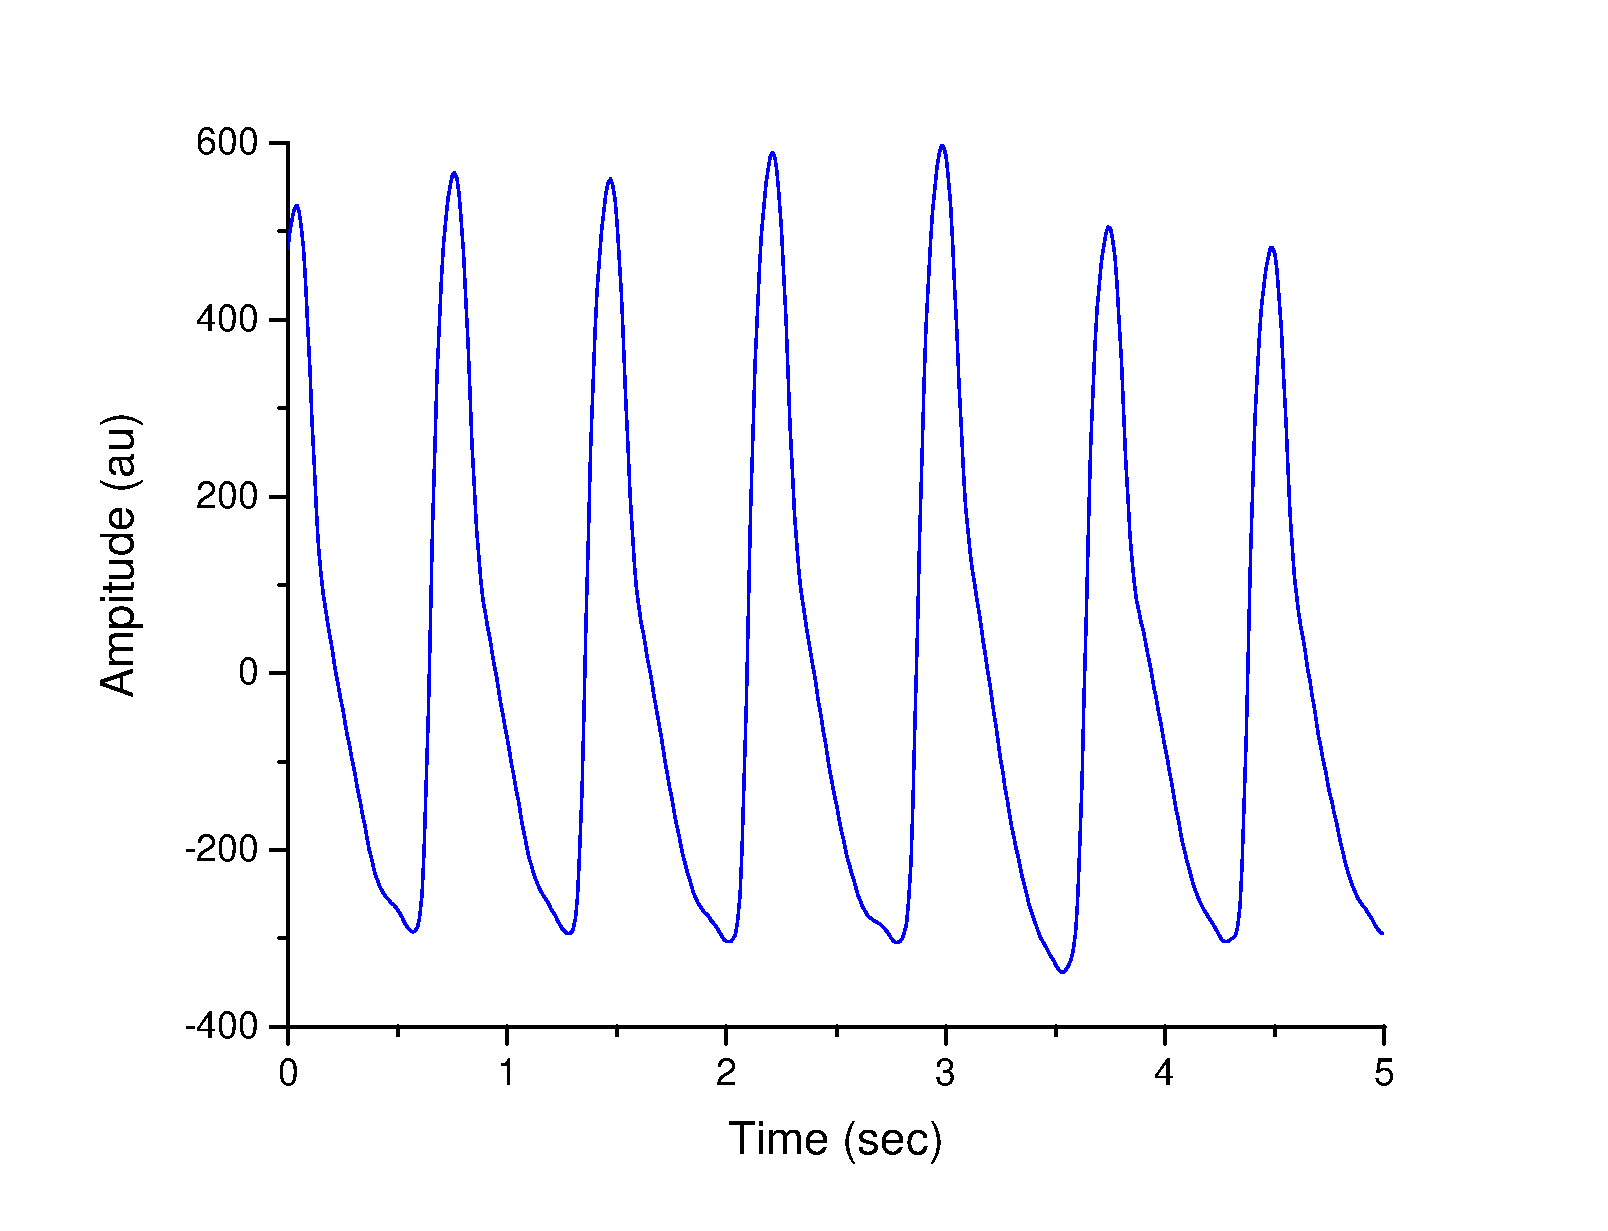
\includegraphics[width=6cm]{pulse_preprocess/before}
    }
    \quad
    \subfigure[平滑滤波后PPG信号]{
    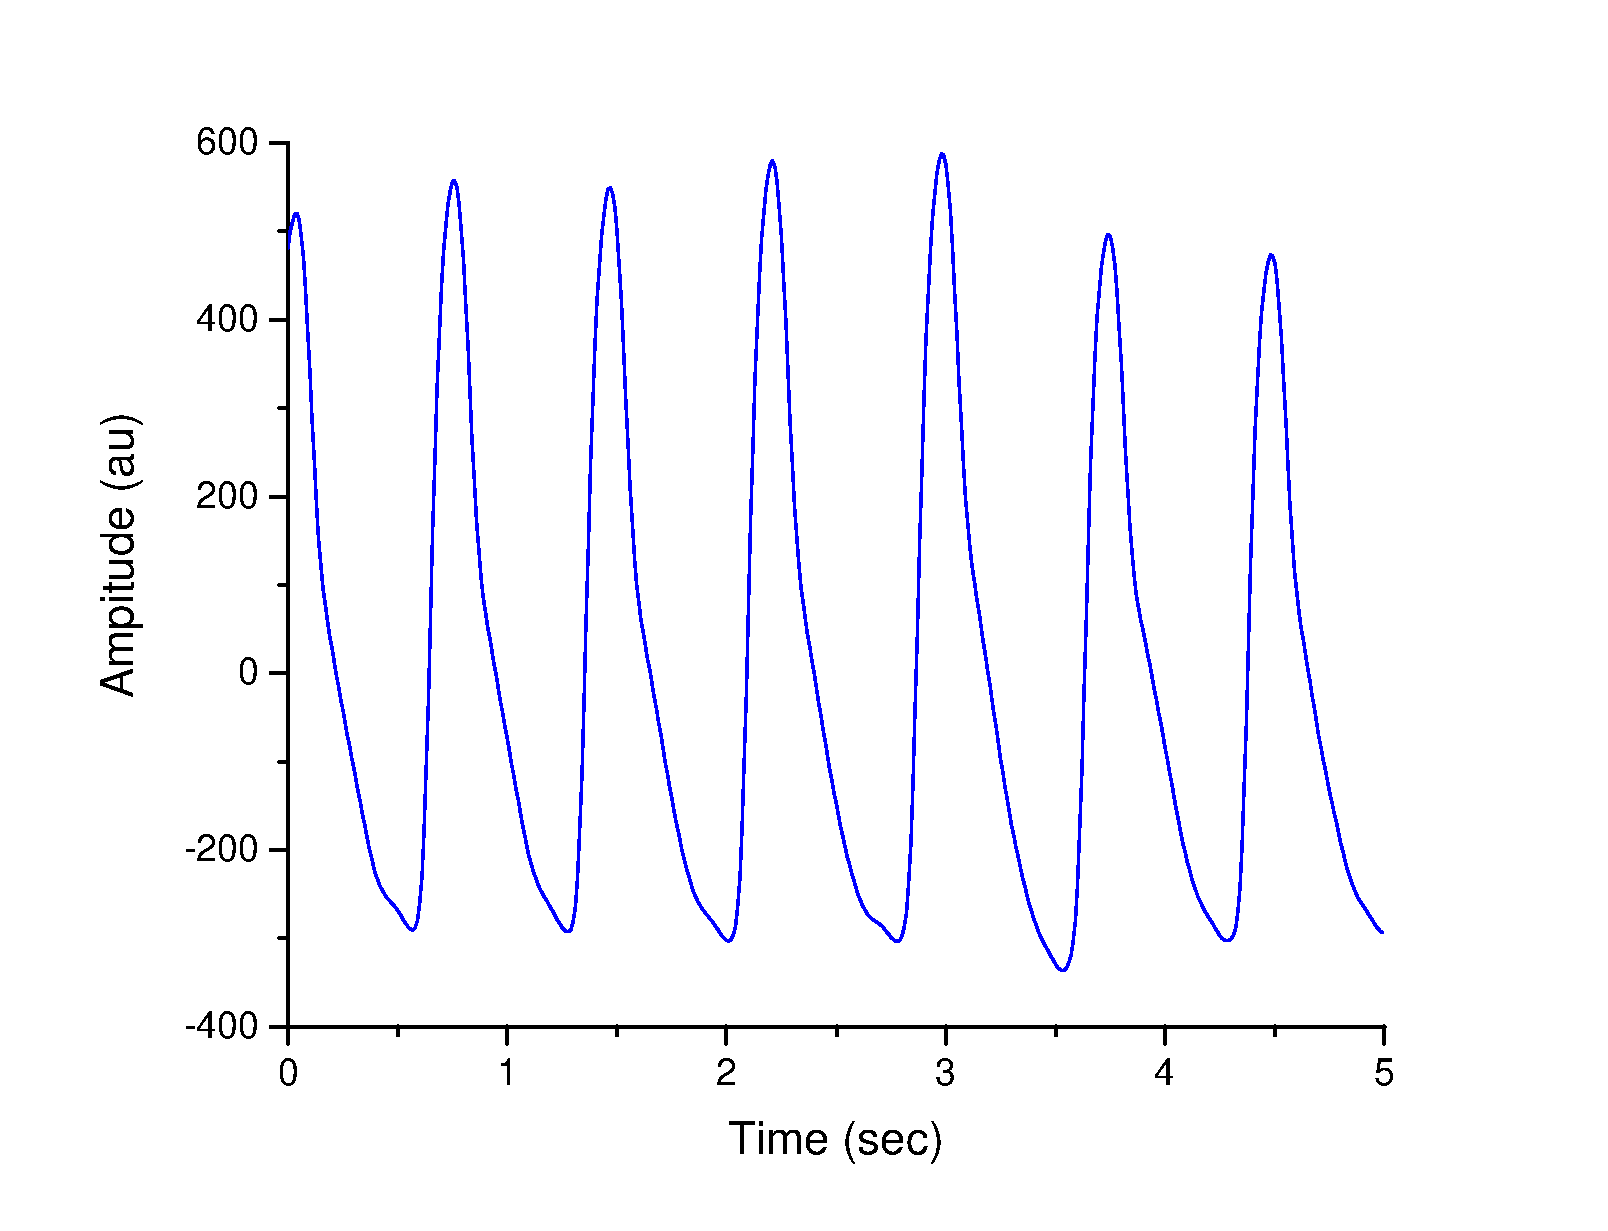
\includegraphics[width=6cm]{pulse_preprocess/after}
    }
    \caption{\label{fig:filter}平滑滤波前后PPG信号对比}
\end{figure}

\subsection{波形检测}
脉搏波波形的正确检测是后续所有特征计算的基础,因此,PPG波形检测算法的准确性及抗干扰能力显得尤为重要。传统的检测算法一般都是对波形进行一次性检测,然后再人工判别检测的准确性。
这种检测算法在应对较为复杂的信号时检测性能有所欠佳。
本小节借鉴了计算机科学领域的机制与策略分离的设计思想,
改进了上述PPG波形检测流程,提出了一种新型PPG波形检测算法,即初筛-复核-投票(Screen-Check-Vote,SCV)算法。

机制与策略分离是计算机系统领域的一项重要设计原则,被广泛应用于一系列资源分配问题(如CPU调度、内存分配、服务质量)以及软件抽象的设计等问题中\cite{Wulf1974,Levin1975,Brinch2001}。
这里的机制可以理解成决定如何做(how),而策略则决定具体做什么(what)。
SCV算法在对PPG波形进行检测时,充分利用“宽进严出”的筛选原则,预先设计了初筛、复核及投票等机制,而对每个机制下具体使用的策略不做过多限制,可有效增强对复杂信号的处理能力、提高算法的检测准确度,
同时极大地保证了算法的适配性与调整的灵活性,这一过程如\autoref{fig:detect}所示。
\begin{figure}[htbp]
    \centering
    
\includegraphics[width=\linewidth]{pulse_preprocess/detect}
    \caption{\label{fig:detect}SCV算法检测流程示意}
\end{figure}

在本研究中,SCV算法主要依据PPG波峰的局部最大值原理进行波形初筛,随后创新性地引入了针对PPG波形的多标准二次复核与最终决策确认机制以减少错检发生的概率。
所有初筛得到的“可疑波形”经特定标准复核后均会得到基于该标准的一个输出判定结果。最后,由检测算法的决策模块负责对多个标准的复核结果进行裁决判定,将“可疑波形”判断识别为正确波形或错检干扰段。
以下是各个机制下使用策略的具体介绍。

一、波形检测

波峰与波谷是脉搏波的最基本特征点,也是检测波形其他特征点的基础。顾名思义,波峰是特定PPG波形内的最大值,在其左邻域内PPG幅值单调递增,右邻域内PPG幅值单调递减,则显然波峰与波谷必然是原始数据中的局部极大值与局部极小值点。
故对PPG波形特征点定位可按以下步骤进行。

1. 波峰定位

计算并遍历原始信号的一阶导数$X^{'}$,若出现$X_i^{'}\ge 0$且$X_{i+1}^{'}\le 0$,则说明出现了极大值。此时,定义时长一长一短的两个搜索窗,分别以当前数据点为窗中心,向前后双向检测并返回窗内最大值的位置。
若两个搜索窗的返回结果一致,则说明返回值就是一个波峰点。为防止同一波峰被多次检测,只有与上一成功检测的波峰位置点不同返回值才会被加入波峰缓存数组$Peaks$中。

在实际检测时,常会出现一阶导数在某邻域内多次出现过零点,导致多个极大极小值连续出现。为避免连续调用搜索窗、提高算法效率,本研究针对性进行了以下剪枝优化设计:

\Rnum{1}.采用中心对称搜索窗

窗口进行最大值搜索时是以当前搜索位置中心对称前后双向搜索,实际当第一个过零点出现时,这一邻域内的所有极值点均已被检索过,得到的局部最值已经是该邻域内最值。

\Rnum{2}.合理设置搜索窗时长

结合正常波形的形态特点,本研究将搜索窗时长分别设置为0.1s与0.3s。前者可以直接剔除掉时间跨度过小的局部极值,后者是基于此前PPG波峰与其重博峰时间间隔的经验值,可以保证重博峰点不会被误检为整个波形的波峰。

\Rnum{3}.搜索窗步进值策略调整

若长窗在当前位置$C$以中心沿时间轴延伸方向找到了局部极大值的坐标$L$后,下一次的搜索窗位置可直接从该$L$处开始。具体而言,若此时短窗返回结果$S=L$,则返回值必然是检测得到的波峰位置$P$,下次搜索可直接从波峰后开始;若$S\ne L$,
此时从$C$至$L$再进行搜索已经不可能再更新$L$坐标。而由于长窗搜索必然包含短窗,故下次搜索也可以同样调整检索位置从$L$处开始。

TODO 
figure here

2. 波谷定位

一般而言,在波峰的位置确定之后,波谷的定位相对简单,一种可行的处理思路是将两个连续波峰之间的最小值定义为PPG波形的波谷。但该思路对复杂信号的处理效果欠佳,因为这种处理思路已经默认了所有的波形均已被正确无误地检测出来且
波形之间有连续性,即任意两个波形之间不存在其他干扰段。
因此,本研究对波谷的定位仍然按照先寻找定位再二次确认的思路进行,其中,波谷在满足上述条件的基础上,需要进一步满足其出现位置必须在这两个波峰之间的后半段。
此步得到的PPG波谷位置也被保存至缓存数组$Troughs$中,这一过程如\autoref{alg:troughs_detect}所示。
\begin{breakablealgorithm}
    \caption{PPG波形波谷定位检测}
    \label{alg:troughs_detect}
    \begin{algorithmic}[1] %每行显示行号
        \Require 待检原始数据数组$Points$,原始数据的一阶差分数组$D$,波峰数组$Peaks$
        \Ensure 正常形态下记录脉搏波波谷位置的数组
        \Function {DetectTroughs}{$Points, D, Peaks$}
            \State 初始化$Troughs$
            \For{$i\gets 0,Peaks.length()-1$}
                \State $leastX \gets (Peaks[i].x + Peaks[i+1].x )/2$
                    \For{$j \gets Peaks[i+1].x)-1, leastX$}
                        \If {$D[j-1]<0 \And D[j]\le 0$}
                            \State $lastT \gets Points[j]$
                            \State \textbf{break}
                        \EndIf
                    \EndFor
                \State $Troughs \gets lastT$
            \EndFor
            \State \Return{$Troughs$}
        \EndFunction
    \end{algorithmic}
\end{breakablealgorithm}

3. 完整波形确认

前两步已经分别得到了原始信号中所有波峰与波谷点,此时仅需按照波谷(start)——波峰(peak)——下一波谷(end)组合成完整波形即可。针对某些异常信号,\autoref{alg:troughs_detect}会出现两波峰之间无法有效检出波谷的极端情况。
因此,有必要对可能组合成完整波形的波峰波谷再次进行检查。本研究以PPG波形必定符合一定的时间规则对上述波峰波谷进行了“组合”。参考以往研究对PPG波形对经验统计,最终组合的波形起点与波形终点间期$P_{S2E}\ge 0.4s$,
波形峰值点与波形终点间期$P_{P2E}\ge 0.3s$。换言之,最终经过确认的波形的间期必定在上述数值内。

4. 其他特征点定位

由于波形其他特征点的定位依赖于波形的正确检测,因此,初筛阶段不做除波峰波谷外的其他特征点检测。这些特征点的检测被推迟到SCV算法检测完成后才进行。

二、多标准评估

上述PPG检测算法与此前的诸多研究中的算法性能接近,改进提高有限。具体而言,对质量高的PPG信号有着较好的检测效果,但对类似\autoref{fig:samplesignal}中的异常段仍难以避免错检漏检等情况的出现。
鉴于此,本研究特原创性地引入了对PPG波形对二次审核评估机制,以进一步增加检测算法对各种干扰信号的检测能力、对畸变信号的识别判断能力。

如绪论中所述,PPG信号可以视为平稳随机信号的一种,短时间采样得到的有效PPG波形信号理应具有较高的相似性\cite{Qiu2012}。另外,有效PPG信号与干扰信号、畸变信号在形态特征、统计特征方面均存在较大差异,存在设计算法实现自动区分的理论可行性。
基于以上前提,为使具有且仅具有PPG波形一般特征的初筛“可疑波形”可以通过复核评估,本研究特设计并提出了以下复核标准:

1.能量与功率标准

易知脉搏波的相对幅值$A$是采样时间$t$的函数,将其表示为$A(t)$。参考信号与系统中对信号能量的定义\cite{Alan2019}
\begin{equation}
    \label{equ:energy}
    E=||f(t)||^2=\int_{-\infty}^{+\infty}{|f(t)|^2}\,d t
\end{equation}
类似地,单个PPG信号的能量可表示为
\begin{equation}
    \label{equ:ppge}
    E=\sum_{t=t_{start}}^{t_{end}}|A(t)|^2
\end{equation}
同理可得该PPG波形在其持续时间内的平均功率为
\begin{equation}
    \label{equ:ppgp}
    P=\frac{E}{t_{end}-t_{start}}=\frac{\sum_{t=t_{start}}^{t_{end}}|A(t)|^2}{t_{end}-t_{start}}
\end{equation}
能量与标准标准基于PPG波形在原始采集数值上,即PPG信号中交直流信号成份总和(AC与DC)的相似性。若所有初筛波形的功率求其均值,可得筛选波形的平均功率$P_{mean}$。
本研究规定通过能量标准复核的波形其功率必须在$P_{mean}$的一定倍数区间内$[0.4 \cdot P_{mean},1.8 \cdot P_{mean}]$。

2.方差与标准差标准

若原始PPG信号中DC成份波动较大(如基线严重漂移),会使部分波形功率数值偏离上述正常$P_{mean}$合理倍数区间,导致这部分波形被能量与功率标准错误识别为干扰。因此,本研究引入了方差与标准差标准以重点关注PPG波形AC成份的相似性。
若将特定PPG波形持续时间内所有采样点均值定义为$\mathop{A} \limits^-$,则该波形的标准差可表示为
\begin{equation}
    \label{equ:ppgstd}
    S=\sqrt{\frac{\sum_{i=1}^{n}{(A_i-\mathop{A} \limits^-})^2}{n}}=\sqrt{\frac{\sum_{i=1}^n{A_i}^2}{n}-{\mathop{A} \limits^-}^2}
\end{equation}
类似地,可以计算所有初筛波形的标准差均值为$S_{mean}$。本研究规定通过标准差复核的波形其相应数值必须在$S_{mean}$的一定倍数区间内$[0.4 \cdot S_{mean},1.8 \cdot S_{mean}]$。

3.时间关系标准

时间关系标准是对PPG波形间期、波形上升支与下降支及重博波峰相关特征时长间期做出对限定,是所有合格波形筛查所共有的一般范式。

由于时间标准通常与特征点的联系紧密,部分时间标准已经在
波形定位阶段得到了应用。如波形检测阶段,搜索窗的窗长已经限定了重博波峰与主波峰间期$T_{P2R}\ge0.3s$;
完整波形在进行确认时也限定了波形周期$T_{S2E}\ge 0.4s$、下降支时长$T_{P2E}\ge 0.3s$。
若参照心率定义,将一分钟中内有效脉搏波的数量规定为脉率(Pulse Rate,PR)。那么,原则上该算法可对$PR \le 150$的原始脉搏波数据进行波形检测。

此外,由于血管回流作用,PPG波形的下降支较上升支更长,因此,波峰位置必然在整体的前半段,在此基础上,波峰在波形中的位置可用下式表征
\begin{equation}
    \label{equ:timestd}
    PP = \frac{t_{end}-t_{start}}{t_{peak}-t_{start}}
\end{equation}

为排除异常极值的影响,本研究在计算出所有波形的$PP$数值并按升序排列后,取前$20\%$-$80\%$的波形计算其均值${PP}_{mean}$。
本研究规定通过基线偏移复核的波形其$PP$数值必须在${PP}_{mean}$的一定倍数区间内$[0.8 \cdot {PP}_{mean},1.2 \cdot {PP}_{mean}]$。

4.基线偏移标准

基线偏移最值标准是对PPG波形的起点与终点幅值差异程度的衡量。若两者的差值过大说明基线漂移严重,而这往往意味着波形处于一段较强的干扰中,具有较大的信号畸变可能,如\autoref{fig:samplesignal}所示。
若规定PPG波形起点与终点中幅值的较大的为$A_G$,较小值为$A_L$,同时规定$A_P$、$A_S$与$A_E$分别为波形波峰幅值、起点幅值与终点幅值,则基线偏移程度可用下列公式衡量
\begin{equation}
    \label{equ:baselinestd}
    \left \{
    \begin{aligned}
        \delta B &=A_G-A_L \\
        \Delta B &=\frac{A_G-A_L}{A_P-A_L}=\frac{\delta B}{A_P-A_L}\\
        \Delta B' &=\frac{A_P-A_S}{A_P-A_E}
    \end{aligned}
    \right.
\end{equation}
其中,$\delta B$是对偏移的绝对值的衡量,$\Delta B$与$\Delta B'$则是对偏移程度归一化的衡量。
TODO figure here

由于正常PPG波形$\Delta B$数值较小,而基线严重漂移时$\Delta B$数值显著增大,甚至达到正常波形的数十倍以上。
为消除漂移波形对最终均值的影响,本研究在计算出所有波形的$\Delta B$数值并按升序排列后,取前$80\%$的波形计算其均值${\Delta B}_{mean}$。
本研究规定通过基线偏移复核的波形其$\Delta B$数值必须在${\Delta B}_{mean}$的一定倍数区间内$[0,10 \cdot {\Delta B}_{mean}]$,
类似地,$\delta B$数值必须在${\delta B}_{mean}$的一定倍数区间内$[0,8 \cdot {\delta B}_{mean}]$。
而对$\Delta B'$而言,计算均值再排序的意义不大,由于$A_S$与$A_E$在\autoref{equ:baselinestd}中的对称性,最终数值的上下限必定互为倒数关系,本研究规定的倍数区间为$[0.5,2]$。

5.其他标准

目前为空,待补充。
由于不同人群、不同采集设备、不同采集环境下采集得到的PPG信号可能形态上千差万别,与之对应的干扰信号也往往不尽相同。上述标准仍有不足以甄别区分有效信号与无效干扰的可能。
故在此特保留其他标准占位,供后续研究视情况开发设计新标准从而进行功能性拓展。

三、投票决策

当初检波形经过上述PPG评估标准后,均会生成一定的输出,即基于当前标准判断的正确检测波形或错检干扰。为获取最终的评判结果,需要综合以上多个评估标准的输出,形成最终的裁定。
若将多个学习器$h_i$在样本$x$上的预测输出表示为$N$维向量
\begin{equation}
    \label{equ:vector_h}
    \boldsymbol H(x) = [h_1(x),h_2(x),\cdots,h_N(x)]
\end{equation}
其中,$h_i(x)$的值域为类别标记集合$\{c_0,c_1,\cdots,c_N\}$。
此时,上述评估过程可进一步抽象成
\begin{equation}
    \label{equ:output_h}
    Y(x) = f(\boldsymbol H(x))
\end{equation}
其中,$f$为具体决策策略函数。

在机器学习领域,集成学习(参见本研究第5章相关内容)中的投票策略(voting)给出了了几种决策方法$f$\cite{Zhou2016}。
具体而言,集成学习将上述学习器$h_i$按输出值类型分为了类标记与类概率等两大类。
而基于这两类输出值进行的投票也相应被称为硬投票与软投票,类标记与类概率的特点可总结概括为\autoref{tab:vote}所示。
其中,硬投票可能会导致最终的分类结果由多数概率值较低的学习器决定,而非少数概率更高、更有分类把握的学习器。因此,在条件允许的情况下,应尽可能使用软投票机制进行决策。
本研究在借鉴集成学习常见可用的三种投票策略的基础上\cite{Kittler1998,Zhou2016},重新设计了更符合PPG检波算法的投票决策机制,以下为具体介绍:
\begin{table}[htbp]
    \centering
    \caption{\label{tab:vote}类标记与类概率特点对比}
    \begin{tabularx}{\linewidth}{c|X<{\centering}X<{\centering}}
        \Xhline{1pt} 
            &\textbf{类标记}&\textbf{类概率}\\
        \hline
        \textbf{$h_i^j(x)$值域}  &$\{0,1\}$    &$[0,1]$     \\
        \textbf{$h_i^j(x)$输出说明}&\tabincell{c}{若$h_i$将样本$x$预测为$c_j$\\则取值为1,否则为0}&\tabincell{c}{$h_i^j(x)$相当于对后验概率\\$P(c_j|x)$的一个估计}\\
        \textbf{投票策略}&\tabincell{c}{绝对多数投票法、\\相对多数投票法}&加权投票法\\
        \textbf{别称}    &硬投票 &软投票 \\
        \Xhline{1pt}
    \end{tabularx}
\end{table}

1.绝对多数投票法

绝对多数投票法的决策原则为若某标记得票数超过半数,则预测为该标记,否则拒绝该预测。
\begin{equation}
    \label{equ:mvoting}
    H(x)=
    \left \{
    \begin{aligned}
        c_j,&\quad if \sum_{i=1}^T{h_i^j(x)}>0.5\sum_{k=1}^N{\sum_{i=1}^T}{h_i^k(x)}\\
        reject,&\quad otherwise.
    \end{aligned}
    \right.
\end{equation}

2.相对多数投票法

应用绝对多数投票法时,若对所有标记类别,其得票数均不超过半数,则此时无法得出投票结果。为避免此情况发生,相对多数投票法直接将预测为得票最多的标记。若同时有多个标记获得最高票,则从中随机选取一个作为最终结果。
\begin{equation}
    \label{equ:pvoting}
    H(x)=c_{\arg \max\limits_{j} \sum_{i=1}^T{h_i^j(x)}}
\end{equation}

3.加权投票法

与前面两种投票法不同,加权投票法给所有的学习器$h_i$以特定的权重$w_i$,将所有可能汇总后得到最后的标记类别,
\begin{equation}
    \label{equ:wvoting}
    H(x)=c_{\arg \max\limits_{j} \sum_{i=1}^T{w_ih_i^j(x)}}
\end{equation}
其中,$w_i\ge0$,$\sum_{i=1}^T{w_i=1}$。

4.改良的加权投票法

在实际处理PPG波形的复核时,会出现某几个标准的有着特定的输出组合后(此时可忽略其他所有输出),即可直接判断波形是否异常的情况。另外,标准功率与标准差在定义上就有着极高的相似性,实际检测结果也十分相近,
在与其他标准综合决策前有进一步调整压缩的可能与必要。
基于上述考虑,本研究最终对加权投票的策略进行了一定程度的改良如\autoref{tab:voting}所示。

上文介绍的能量标准、标准差及方差标准等被压缩成三个新的综合标准。
综合标准在进行计算时,使用原标准基于波形是否异常的0或1的输出直接进行数值加法,而非基于各项原始数值。在进行加权投票时,\autoref{tab:voting}中综合标准的类概率是基于本实验数据得到的经验数值,综合标准加权
计算结果超过0.5的波形会被判断为干扰。
\begin{table}[htbp]
    \centering
    \caption{\label{tab:voting}经改良的加权投票法}
    \begin{tabularx}{\linewidth}{X<{\centering}X<{\centering}cX<{\centering}}
        \toprule
        \textbf{综合标准}&\textbf{计算方式}&\textbf{类概率权重}&\textbf{直接判为异常条件}\\
        \midrule
        能量类标准&     $ES=P+S$               &0.3& $ES =2$ \\
        时间类标准&     $TS=PP$&0.2&/\\
        基线类标准&     $BS=\delta B+\Delta B+\Delta B'$&0.5& $BS\ge 2$  \\
        \bottomrule
    \end{tabularx}
\end{table}

四、检测算法性能评估

SCV算法并不保证检测波形在时间上的连续性,在初筛阶段就会忽略明显不符合时间标准的PPG数据段,而肉眼可辨别的明显异常的波形也在复核阶段被检测出来。
此外,由于实际中对异常的波形的漏检的代价远高于对正常波形的漏检,因此,SCV算法在设计时便对异常波形及其前一个波形一并视为异常处理,这可能会导致某些漏检的发生。
为精确评估本研究提出的PPG波形的SCV算法的性能表现,这里以本次研究得到的实验数据及公开数据库的PPG数据分别对其进行了测试。

1. 基于本次实验数据

如第二章中所述,本次实验共采集到有效数据79条,经统计分析,最终得到有效PPG波形共计7864个。而使用SCV算法对其进行检测,结果显示,SCV算法共计错检波形26个、漏检波形7个,
整体的准确率高达$99.6\%$以上。
\autoref{fig:detect_details}给出了展现SCV算法优异的检测性能的一些典型案例。由于篇幅所限,更多典型案例可参见\pageref{fig:detect_details2}页附录A。
此外,\pageref{fig:detectcheck}页附录B也给出了展现SCV算法具体检测过程的一个详尽实例。
\begin{figure}[h]
    \centering
    \subfigure[\label{fig:c_cll}被试CLL的波形检测结果(局部)]{
        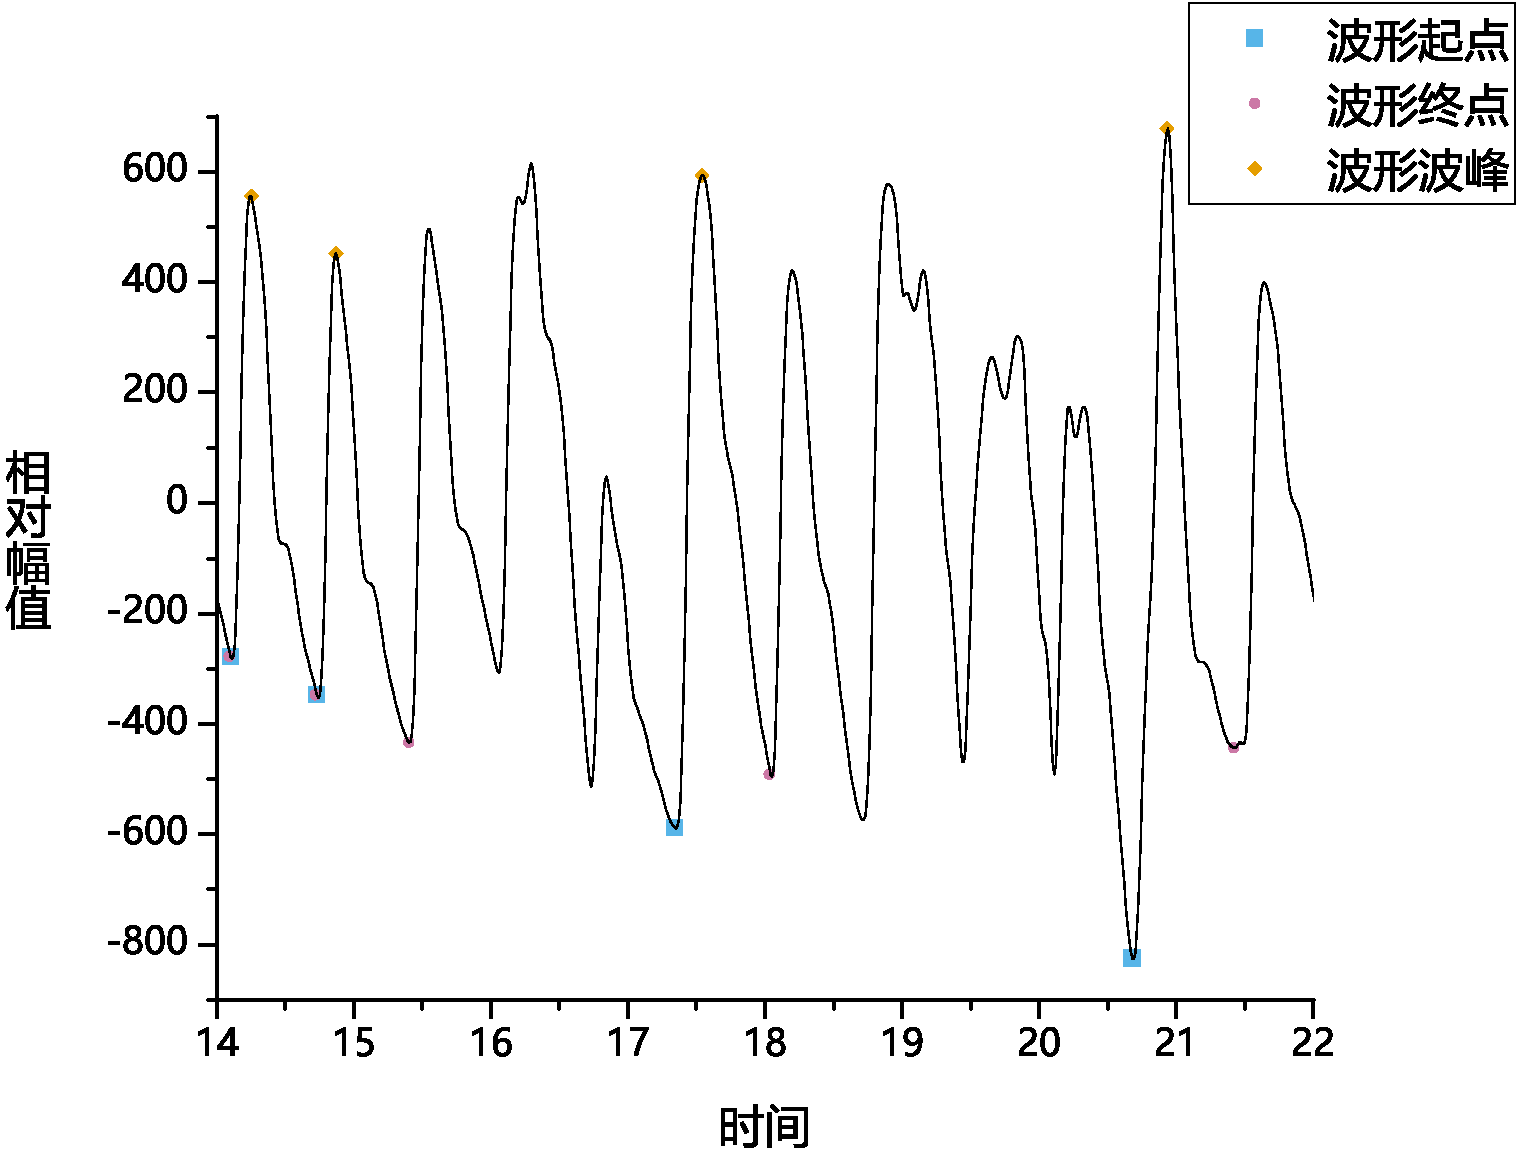
\includegraphics[width=7.5cm]{pulse_preprocess/check/cll}
    }
    \quad
    \subfigure[\label{fig:c_cww}被试CWW的波形检测结果(局部)]{
        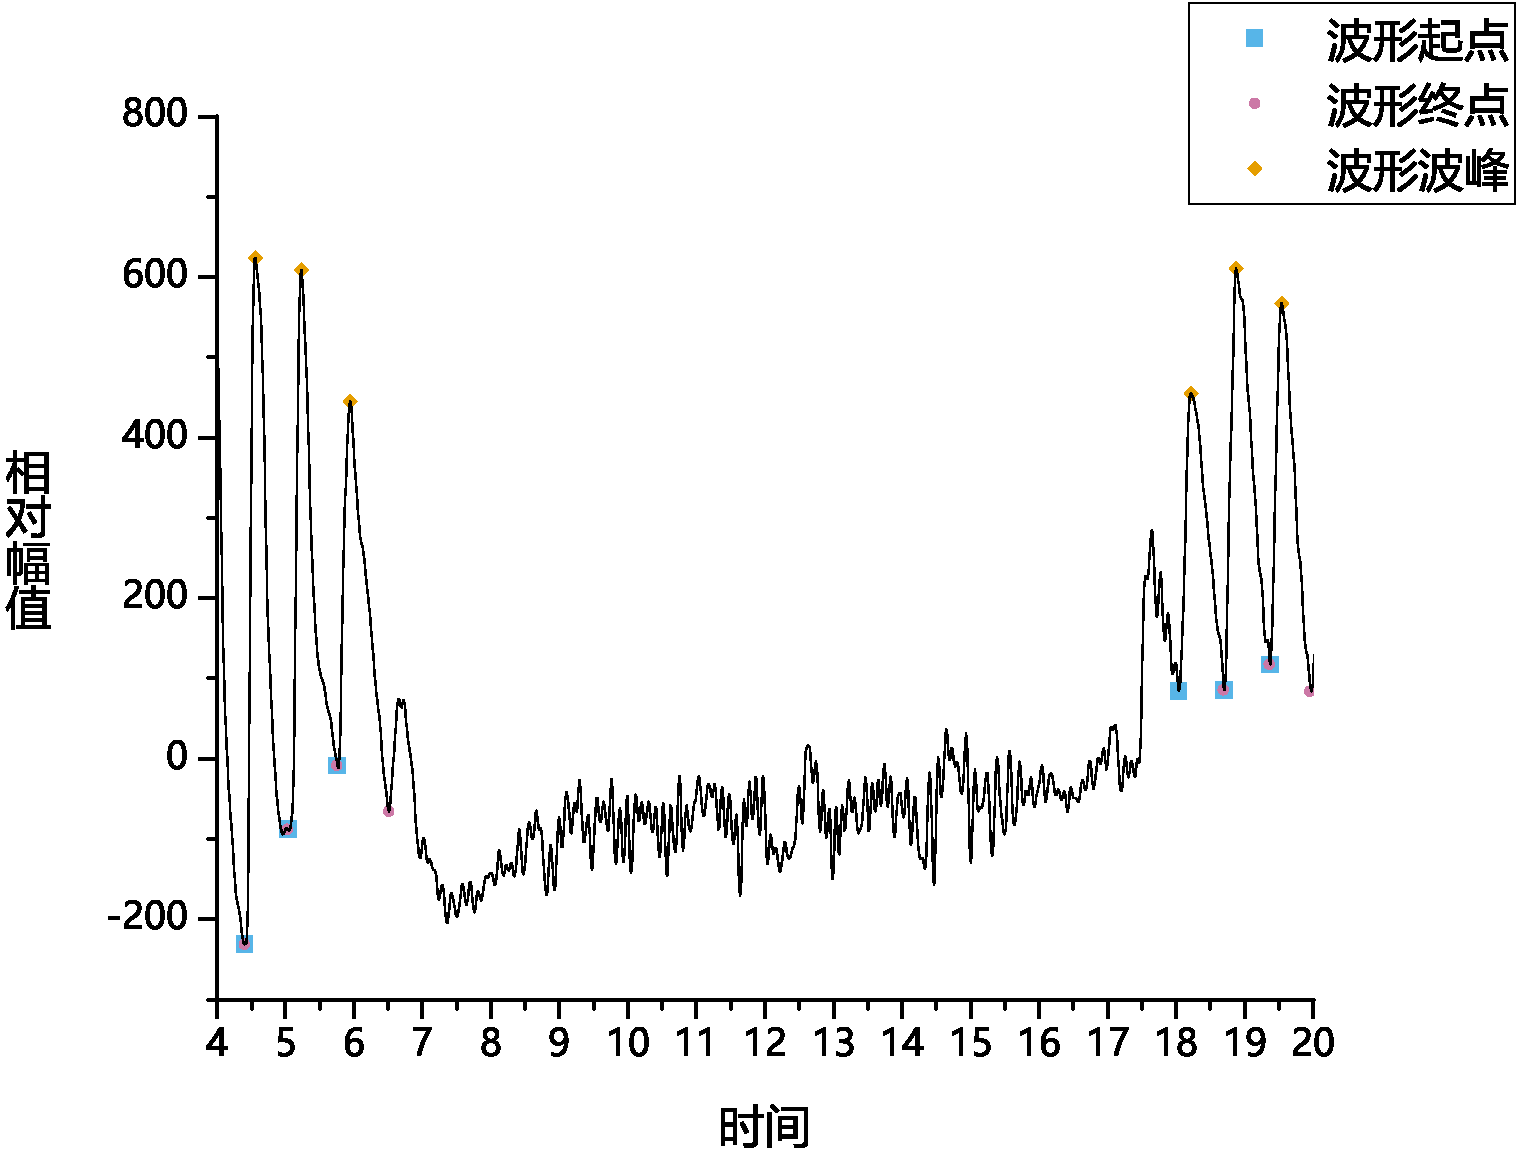
\includegraphics[width=7.5cm]{pulse_preprocess/check/cww}
    }
    \quad
    \subfigure[\label{fig:c_flh}被试FLH的波形检测结果(局部)]{
        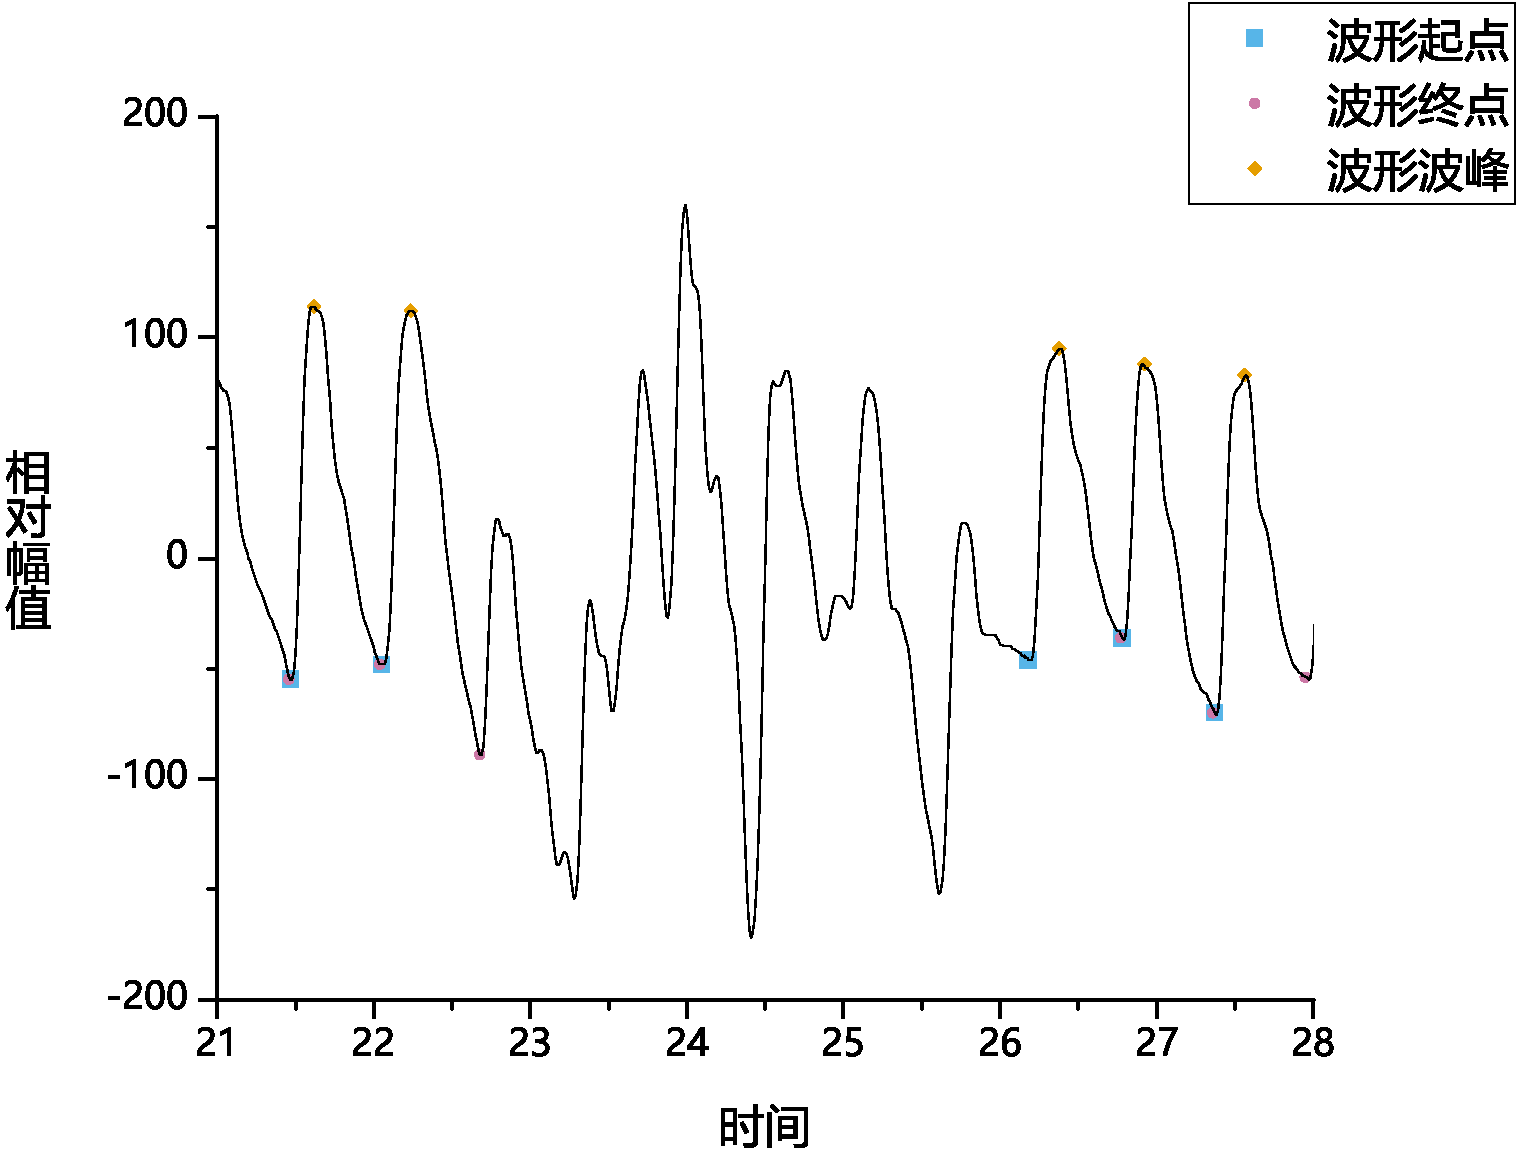
\includegraphics[width=7.5cm]{pulse_preprocess/check/flh}
    }
    \subfigure[\label{fig:c_ly}被试LY的波形检测结果(局部)]{
        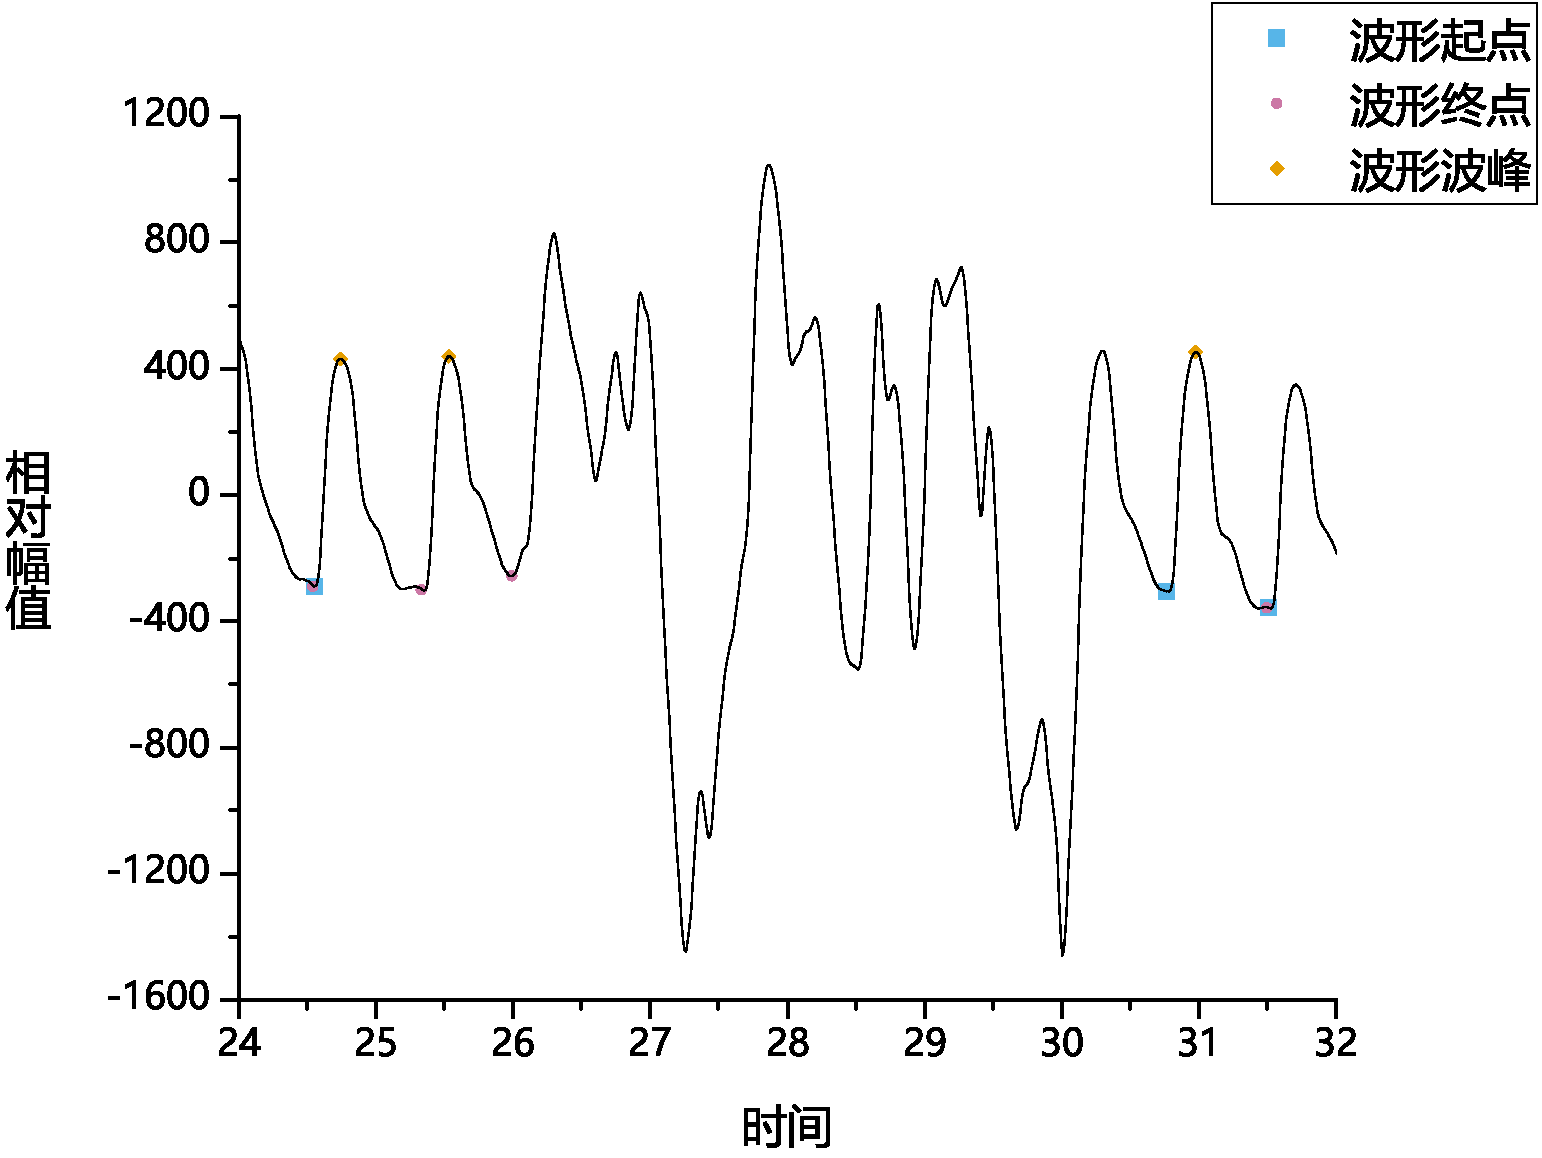
\includegraphics[width=7.5cm]{pulse_preprocess/check/ly}
    }
    \quad
    \caption{\label{fig:detect_details}SCV算法对复杂信号的检测效果示意}
\end{figure}

2. 基于公开数据库UCI-BP

MIMIC(Medical Information Mart for Intensive Care)是生物医学工程领域开源社区PhysioNet上最为知名的一个大型公开数据库\cite{mit2022,Goldberger2000,johnson2018mimic}。该数据库记录了2001年
至2019年期间贝斯以色列女狄肯斯医疗中心重症监护病房患者的相关数据,拥有超过40,000名患者的医疗健康数据记录\cite{johnson2018mimic}。目前,其最新版本为2022年6月发布的MIMIC-IV v2.0\cite{mimic4}。
2015年,Kachuee Mohamad等人在MIMIC-II的基础上进行了二次开发,他们在原始信号的基础上进行了一定的预处理与数据清洗,构建了无袖带血压估计验证数据集即UCI-BP数据集\cite{Kachuee2015,ucibp2022}。
UCI-BP数据集一共包含12,000条数据记录,每个记录包含脉搏波、有创动脉血压及心电等三通道数据,采样率均为$125Hz$,单条数据记录时长从1分钟内至10分钟不等。
UCI-BP数据集由于其出色的易用性而被广泛使用,本研究亦采用该数据集进行SCV算法的评估与验证。

由于UCI-BP数据记录量大,这里仅以该数据集来自\path{Part_1.mat}文件的前50条数据记录进行了SCV算法的性能评估。在不调整此前SCV算法涉及的各参数的基础上,使用SCV算法这部分数据其进行检测验证。
最终得到有效PPG波形共计17562个,而错检波形仅有50个,整体的准确率高达$99.7\%$以上,其中,共有35条数据记录实现了$100.0\%$的检测率,占参与验证的数据量的$70.0\%$。
这部分数据的统计详情及典型检测案例参见\pageref{tab:ucibp_details}页附录C。

值得一提的是,由于UCI-BP数据集本身包含了某些重症监护下的特殊病人,部分PPG数据异常畸形,已经明显异于正常波形,SCV算法对这部分异常数据的检测能力有限(或者说SCV算法“成功地”将这些畸形波形识别为异常),
如\autoref{fig:ucibp_abnormal}所示。
\begin{figure}[h]
    \centering
    \subfigure[\label{fig:c_0179}编号0179原始数据波形(局部)]{
        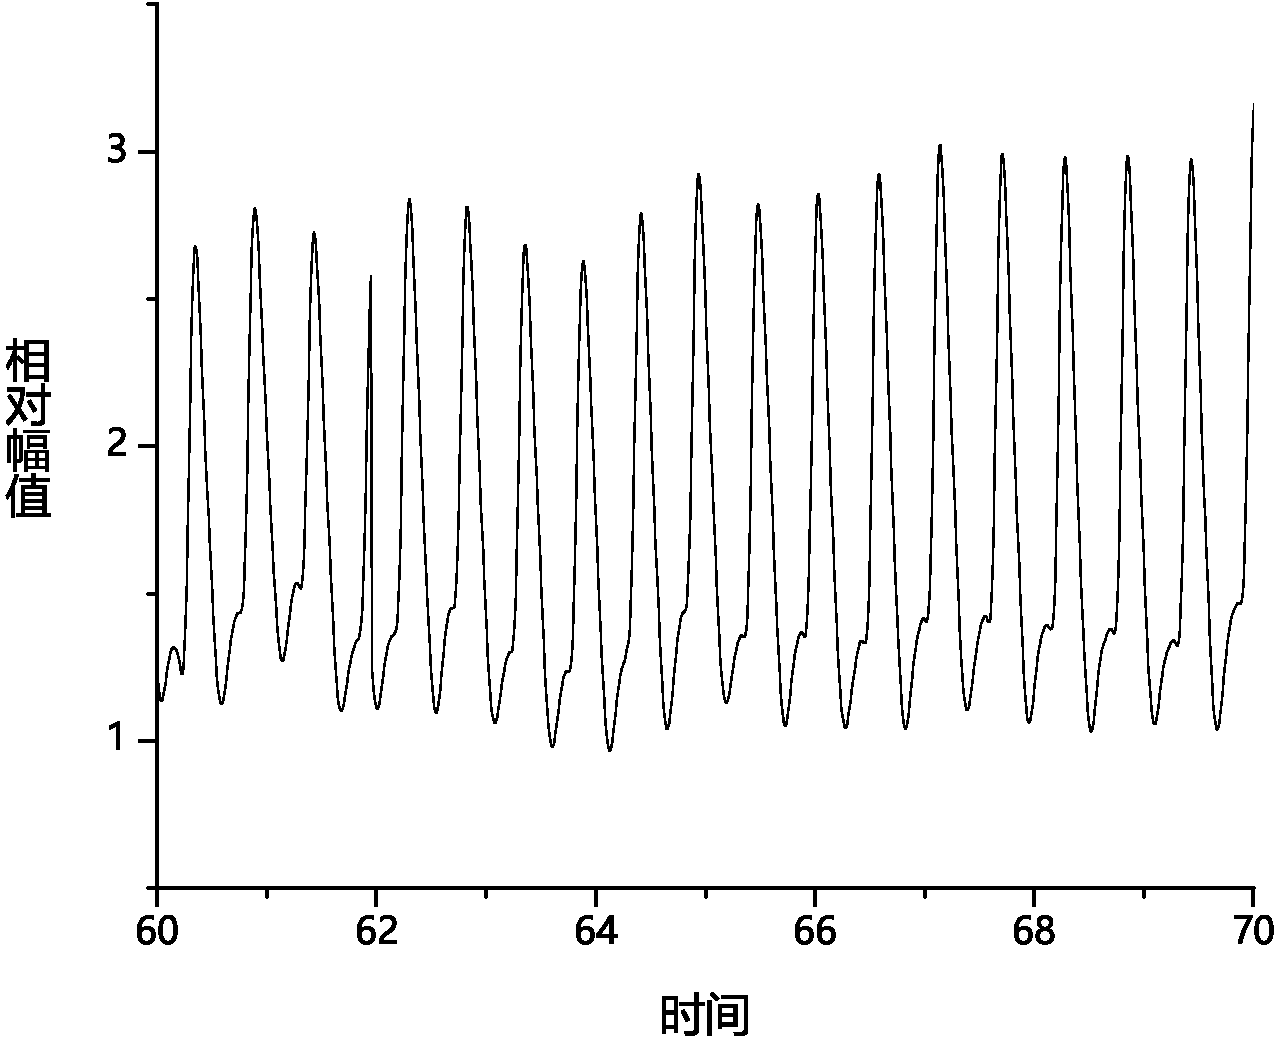
\includegraphics[width=7.5cm]{pulse_preprocess/check/0179}
    }
    \quad
    \subfigure[\label{fig:c_0533}编号0533原始数据波形(局部)]{
        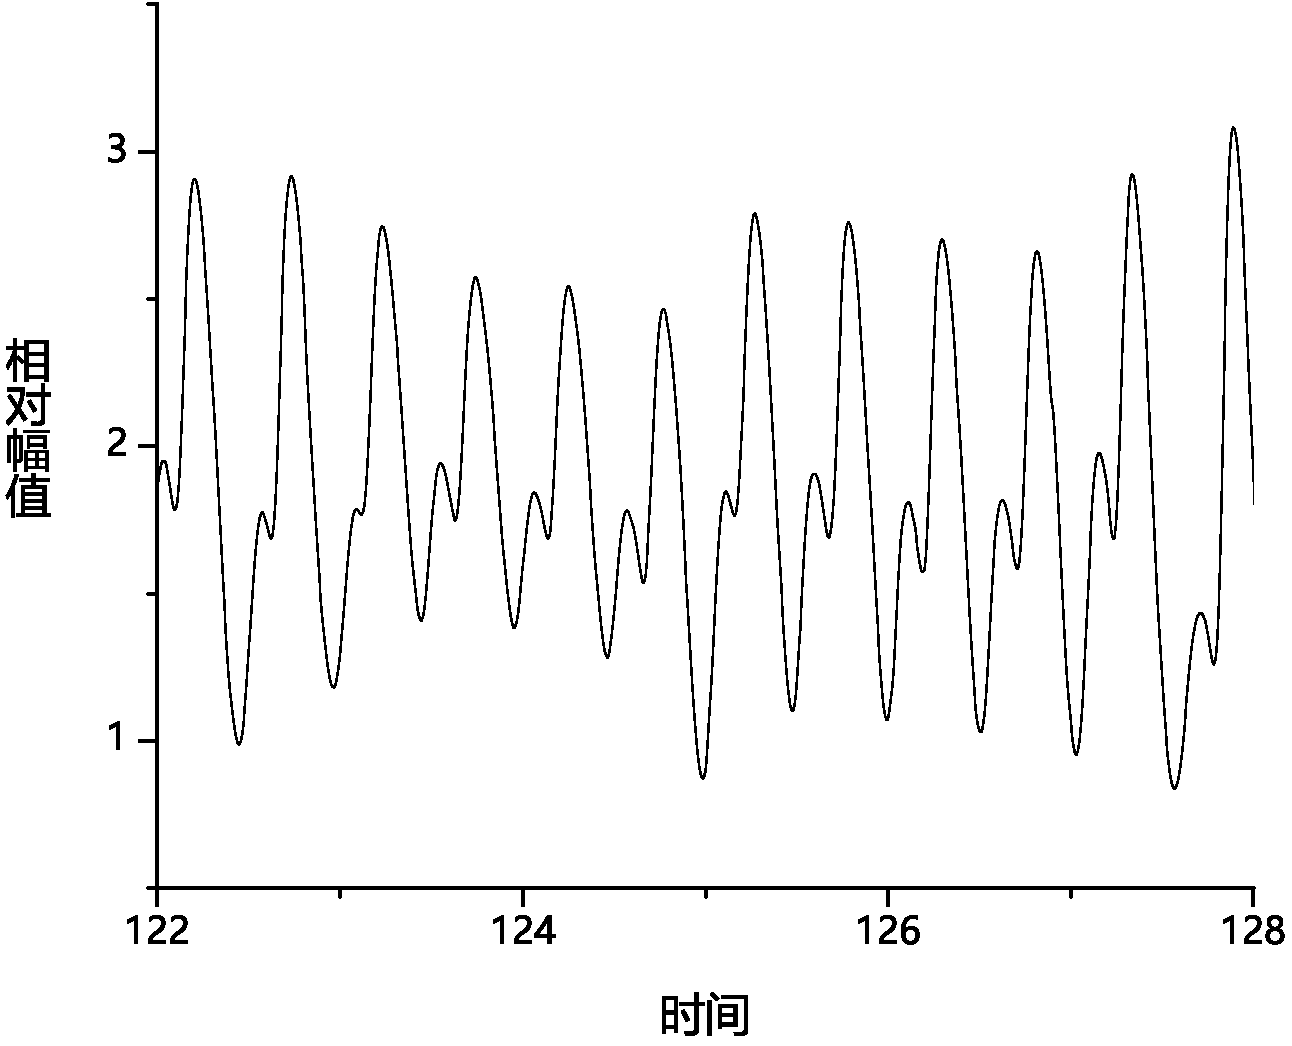
\includegraphics[width=7.5cm]{pulse_preprocess/check/0533}
    }
    \quad
    \caption{\label{fig:ucibp_abnormal}UCI-BP数据库中畸形信号示意}
\end{figure}

五、改进与拓展

针对具体环境下的PPG信号检测,SCV还可以从以下方面做出改进与拓展:

1. 检测算法的改进

初筛阶段现阶段使用的算法可能对某些特殊的信号检测性能欠佳(如\autoref{fig:ucibp_abnormal}),此时可视具体情景进行调整改进。

2. 复核指标的拓展

SCV算法在进行设计时无法穷极模拟各种类型的干扰信号,现阶段的复核指标无法做到对所有干扰的识别,因此,可在必要时重新设计出更能概括异常干扰与正常波形之间差异的新的复核标准。

3. 决策方法的设计

从机器学习的角度来看,脉搏波波形检测SCV算法本质上也是一个二分类的分类器,各个复核标准是用来区分异常与有效波形的输入“特征”,各复核标准的输出即为一个简单二分类器的输出,而最终的
决策输出即为综合多个二分类学习器得到最终输出。因此,在原则上可以借鉴集成学习中的相关算法及设计思想对现阶段的使用的加权投票决策方法进行改进升级。经过数据训练得到的决策模型的参数理论上会比现阶段
直接设置参数数值来决策对实际数据有更好的分类效果。

4. 异常信号的保留取舍

现阶段的SCV算法对于检测得到的异常信号是全部舍弃的,但在某些情景下,可能异常信号可能蕴含着更多信息,是相应研究的重点。因此,SCV算法可拓展成具有可配置选项,自由选择
输出特定类型的波形或更具体的满足特定复核标准的输出的波形。

5.用于其他生理信号的检测

SCV算法是针对脉搏波的检测而设计,但其检测思路也可作为其他人体电生理信号检测算法设计时的参考,可在进行其他信号类似的检测任务时进行一定的移植与改造。

六、综合评价

综上所述,SCV算法在PPG波形检测问题上的检测性能优异,抗干扰能力强。其中,SCV算法复核阶段采用的功率、标准差、时间与基线等四类复核标准
设计合理,均可按照设计初衷识别出特定的异常干扰段,达到数据分析预期。另一方面,由于SCV算法整体采用模块化设计,各模块均具有良好的拓展性,
不论是对已获取的数据进一步提高检测性能,还是对新的存在特定干扰待检信号的准确检测,SCV算法都有着可进一步挖掘的潜力。

\subsection{重搏波与切迹检测}
重博波是脉搏波最具标志性的波形特征之一,其波峰与切迹的检测是一个完整的脉搏波检测算法必不可少的定位项之一\cite{Wang2012}。但在实际应用中,并不是每个人的PPG信号都有着明显的重搏波,特别是当被试出现外周阻力增加、血管壁弹性下降的情况后\cite{mmt}。
此时,随着PPG波形向外周传播,尖锐的重搏波切迹(incisura)常会变形甚至丢失,退变成一简单拐点,甚至重搏波波峰都会在下降支中不显著,导致最后无法从采集得到的信号中对两者直接进行精准定位,如\autoref{fig:samplesignal}所示。

由于本次实验数据中有大量重博波及切迹不明显的信号段,因此本研究借鉴了王选等人于2012年提出的一种基于曲率$K$(curvature)的定位算法对上述特征点进行检测\cite{Wang2012}。
该算法的核心思想是PPG信号在切迹退化成的变形点的邻域内具有最大的曲率值,如\autoref{fig:incisura}所示。
数学中将一般曲线函数在点$(x,y)$处的曲率$K$定义为
\begin{equation}
    \label{equ:curvature}
    K=\frac{|y^{''}|}{{(1+{y^{'}}^2)}^{3/2}}
\end{equation}
其中,$y^{'}$与$y^{''}$分别是曲线函数在该点的一阶导数与二阶导数。王选等人的算法检测过程可概括如\autoref{alg:incisuras_detect}所示\cite{Wang2012}。
\begin{figure}[htbp]
    \centering
    \subfigure[重博波明显的PPG波形]{
    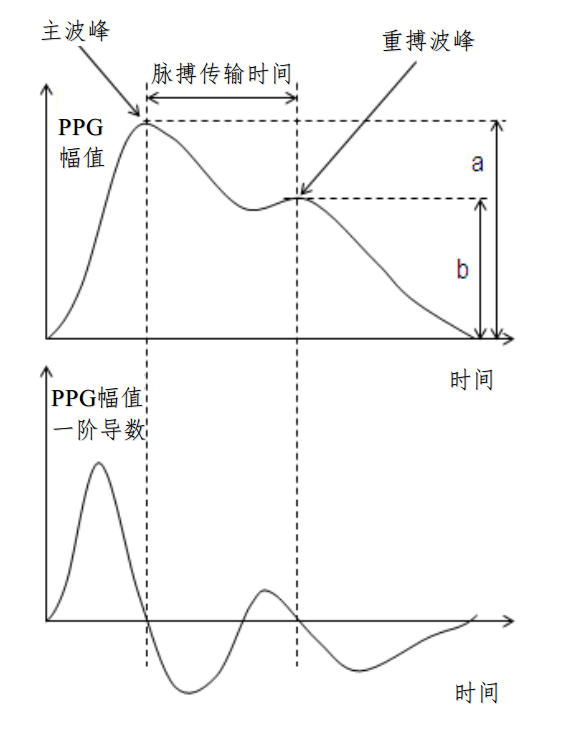
\includegraphics[width=5.5cm]{pulse_preprocess/ri1}
    }
    \quad
    \subfigure[重博波不明显的PPG波形]{
    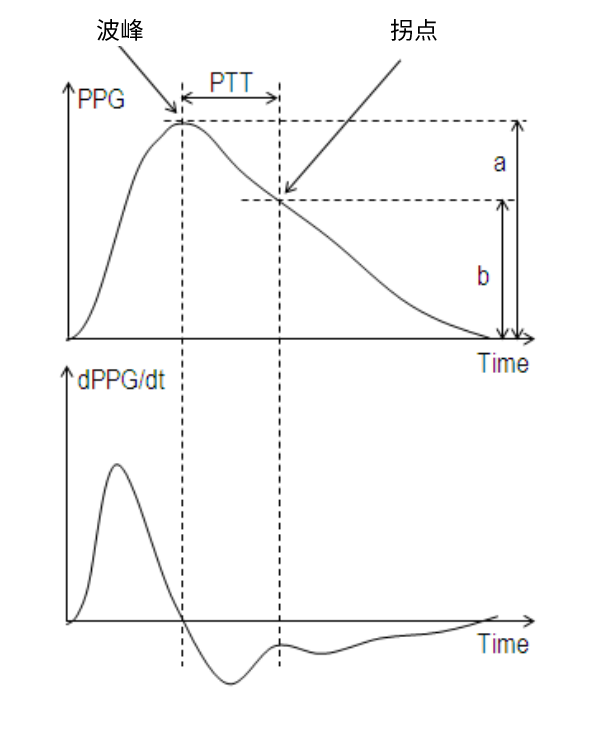
\includegraphics[width=5.5cm]{pulse_preprocess/ri2}
    }
    \caption[重搏波及切迹定位原理]{\label{fig:incisura}重搏波及切迹定位原理\cite{Wang2012,Su2014}}
\end{figure}

\begin{breakablealgorithm}
    \caption{PPG波形切迹定位检测}
    \label{alg:incisuras_detect}
    \begin{algorithmic}[1] %每行显示行号
        \Require 原始数据数组$Points$,检测完毕的波形$pulse$,原始数据的一阶差分数组$D$
        \Ensure 当前波形的切迹位置
        \Function {DetectIncisura}{$Points, pulse, D$}
            \State $s \gets pulse.peak.x + \frac{3}{10}(pulse.trough.x-pulse.peak.x)$
            \State $e \gets pulse.peak.x + \frac{9}{10}(pulse.trough.x-pulse.peak.x)$
            \State \Comment 切迹可能出现的位置为波形的下降支中后部分。
            \State $M  \gets \Call{Max}{$D[s],D[e]$}$
            \State \Comment 寻找到上述区间内一阶导数最大值点记为$M$。
            \If{$D[M] >0$}
                \State \Comment 下降支中存在明显的重搏波。
                \State $Incisura \gets \Call{Min}{Points[s],Points[M]}$
                \State \Comment 重搏波波峰即为点M至脉搏波终点之间的极大值点,切迹为脉搏波波峰至点M之间的最小值点。
            \Else
                \State \Comment 下降支一直单调下降,不存在明显的重搏波。
                \State $Incisura \gets \textproc{Min}({\Call{Curvature}{Points[M],Points[e]}})$
                \State \Comment 重搏波波峰定义为点M至脉搏波终点之间的曲率最大处,切迹定义为脉搏波波峰至点M之间的曲率最小处。
            \EndIf
            \State \Return{$Incisuras$}
        \EndFunction
    \end{algorithmic}
\end{breakablealgorithm}

\subsection{去除基线漂移}
由于呼吸干扰等原因,实际得到的PPG波形的两个波谷的幅值(即该波形的始末位置的幅值)很难保持一致。这种差异最终会导致PPG信号的基线出现波动漂移,如\autoref{fig:drift}所示。为满足后续特定PPG形态特征计算需求,
需要消除基线漂移的影响。此时可借助一种基于线性变换的思路完成相应处理。
\begin{figure}[htbp]
    \centering
    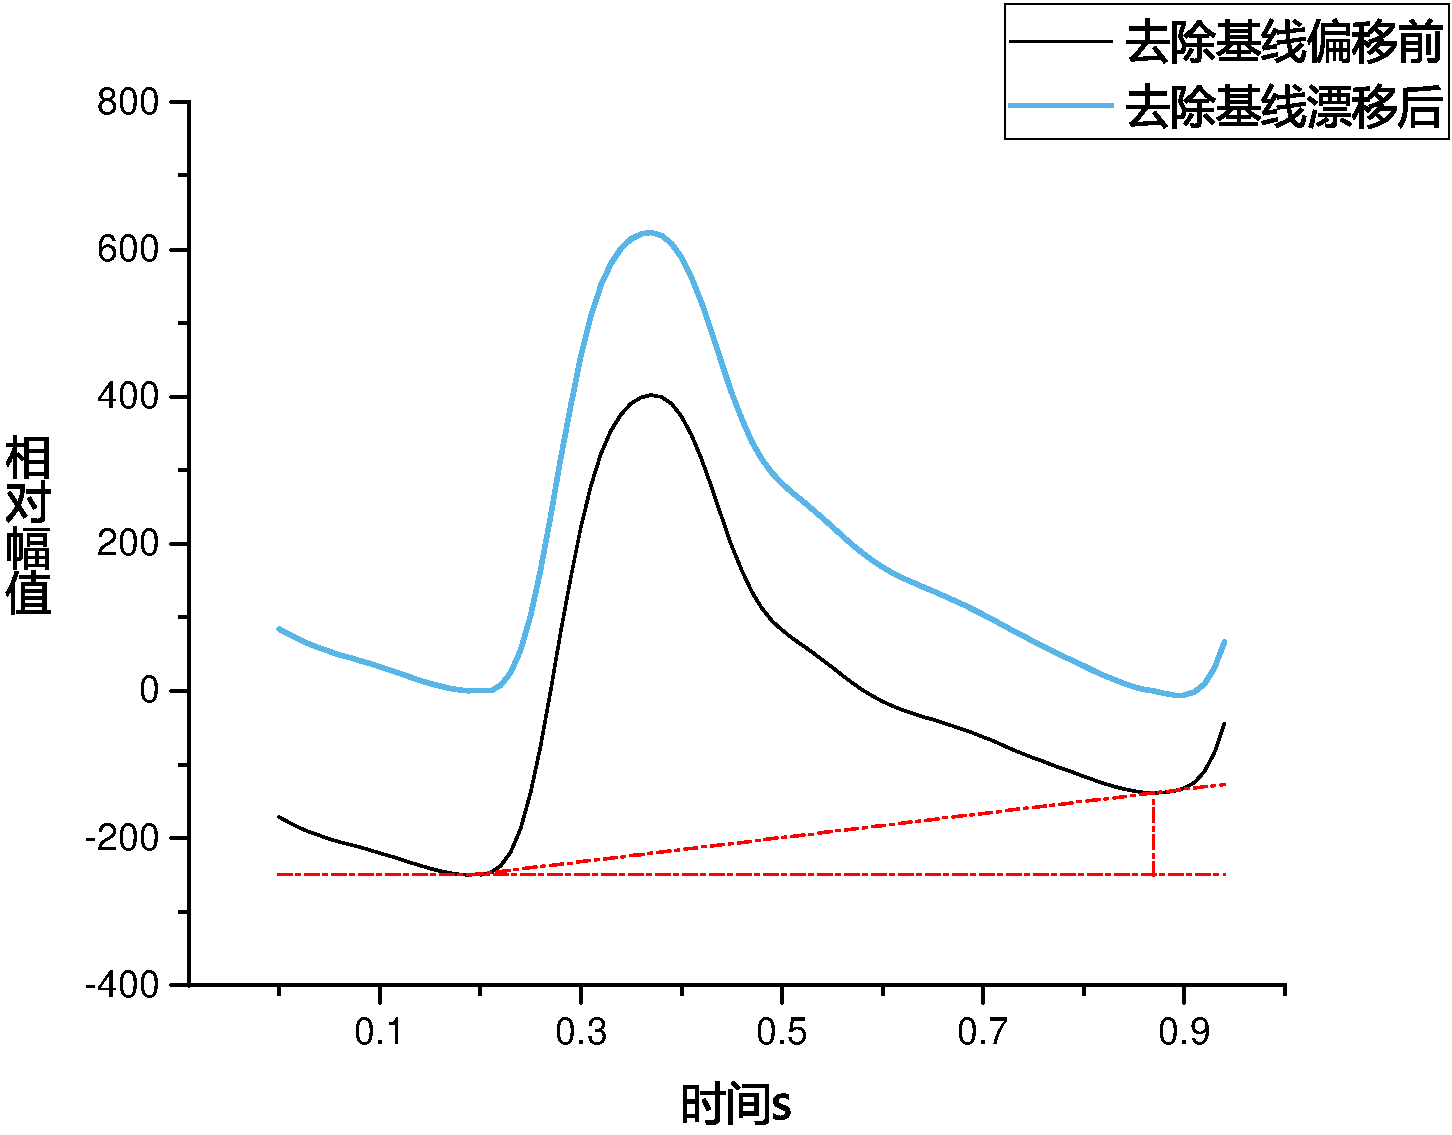
\includegraphics[width=.6\linewidth]{pulse_preprocess/baselineadjust}
    \caption{\label{fig:drift}基线漂移去除原理示意及处理前后对比}
\end{figure}

易知脉搏波的相对幅值$A$是采样时间$t$的函数,将其表示为$A(t)$。对任一特定波形,其起始点与终止点处对应的幅值可分别表示为$A(t_{start})$与$A(t_{end})$。
由于始末位置脉搏波幅值不等,则明显两者之间存在一条斜率$k \ne 0$的直线,其中
\begin{equation}
    \label{equ:linek}
    k=\frac{A(t_{start})-A(t_{end})}{t_{start}-t_{end}}
\end{equation}
则该直线上任意点即代表了在该时刻脉搏波波形与水平基线的偏移量,即
\begin{equation}
    \label{equ:liney}
    \Delta(t)=k(t-t_{start})+A(t_{start})
\end{equation}
此时,去除基线漂移后的脉搏波信号可标示为
\begin{equation}
    \label{equ:adjusta}
    A_{adjsut}(t)=A(t)-\Delta(t)
\end{equation}

\subsection{信号的抽取与插值}
通常而言,脉搏波数据的采样率是固定不变的。但在某些情况下,原始数据采样率不能满足实际需求,在进行相应数据处理任务前需要先进行采样率调整。
如在本研究自行定义设计的多种新型脉搏波时域特征的计算时,经由GE B450设备导出的原始脉搏波数据的采集频率仅为100$Hz$,难以满足后续计算看,需要进行额外处理以提高信号采样率。
其中,减少抽样率的过程称为信号的抽取,也称抽样率压缩;增加抽样率的过程则称之为信号的插值,也即抽样率扩张\cite{Cheng2008}。信号的抽取与插值都会导致原始信号出现频谱迁移,即改变信号的频率成份\cite{Cheng2008}。

相对而言,信号的抽取过程更容易理解。若需要用整数$D$对$x(n)$进行抽取,以使抽样率降低到原始值的$1/D$,可按照每连贯的$D$个抽样中取出一个信号值。这样的处理称为整数$D$抽取\cite{Cheng2008}。
插值是抽取的逆过程,通过某些已知的数据点去推断一个(系列)特定的函数,使得所有已知数据点均在该函数图像上,从而去推断更多未知数据点,这一过程如\autoref{fig:spline}所示。若不考虑可能出现的信号失真,理论上
可以通过调整抽取与插值的数值对原始信号的采样率进行任意的调整。
\begin{figure}[htbp]
    \centering
    \subfigure[经过点(1,2),(2,1),(4,4)和(5,3)的线性样条]{
    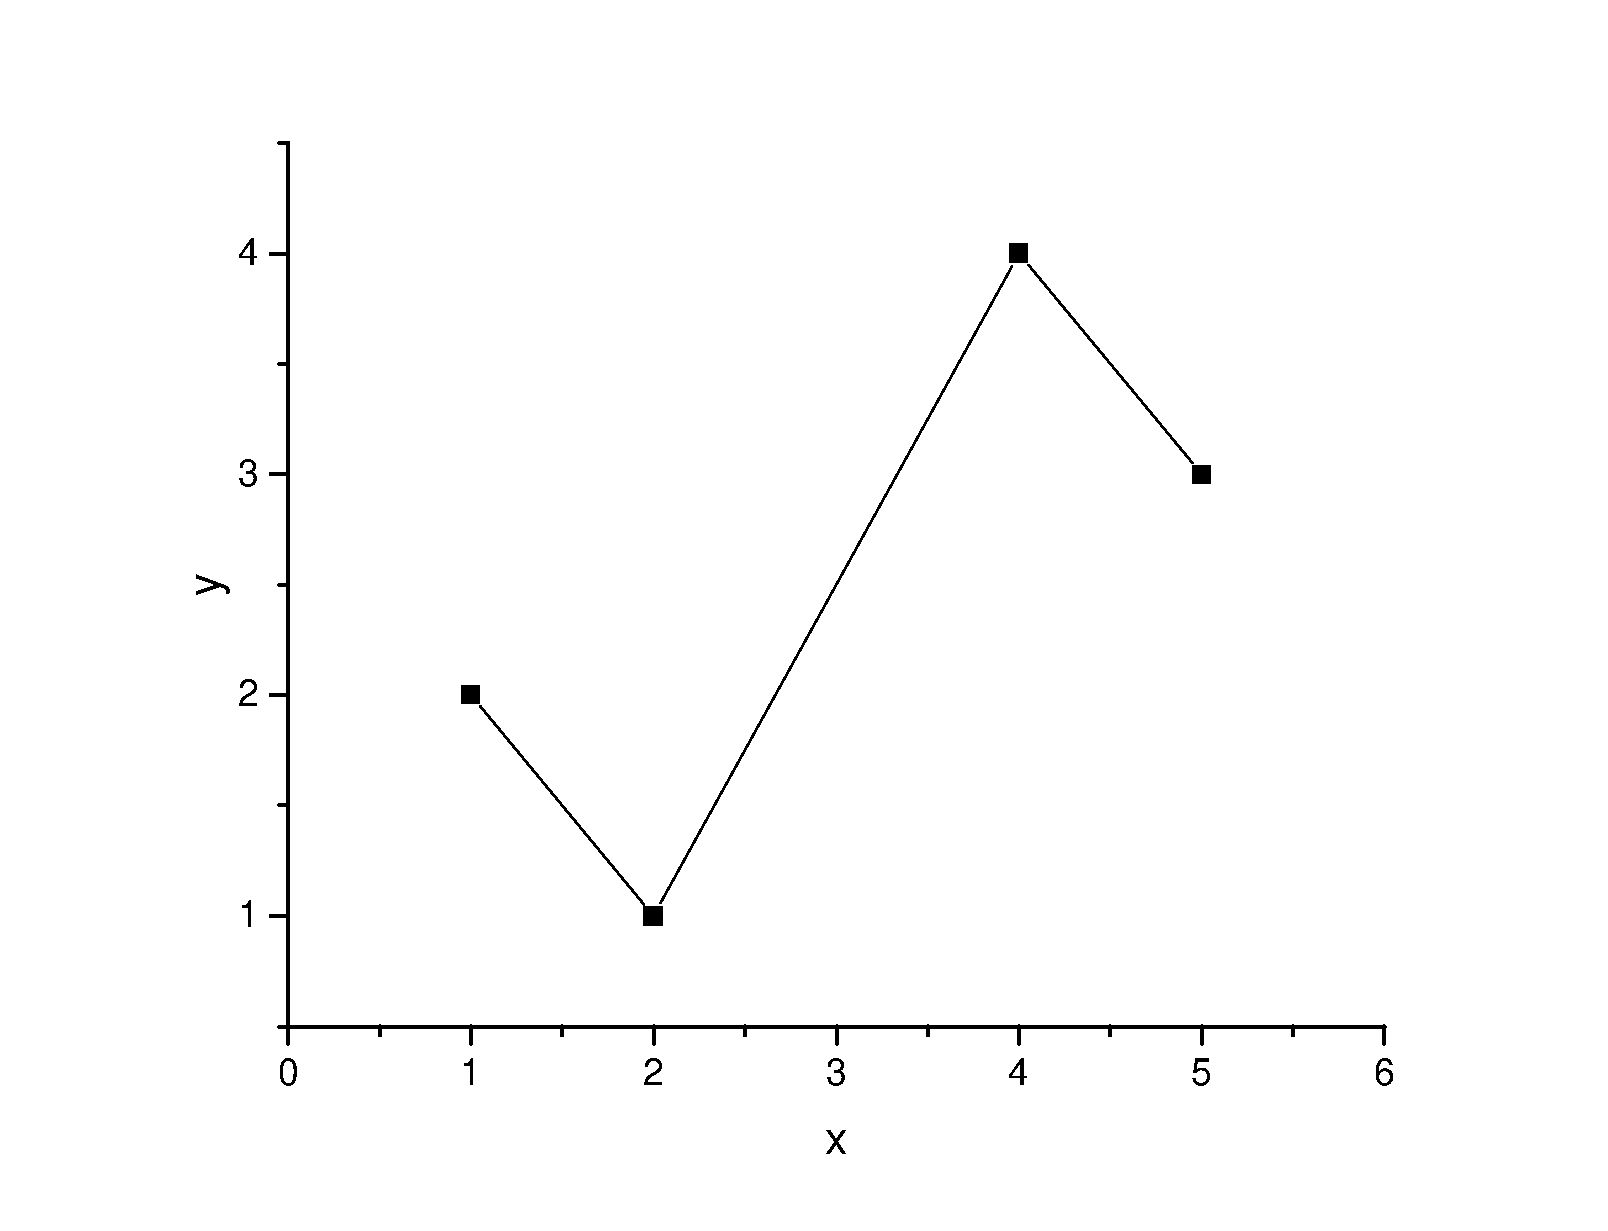
\includegraphics[width=5.5cm]{pulse_preprocess/spline1}
    }
    \quad
    \subfigure[经过相同点的一种可能的三次样条插值]{
    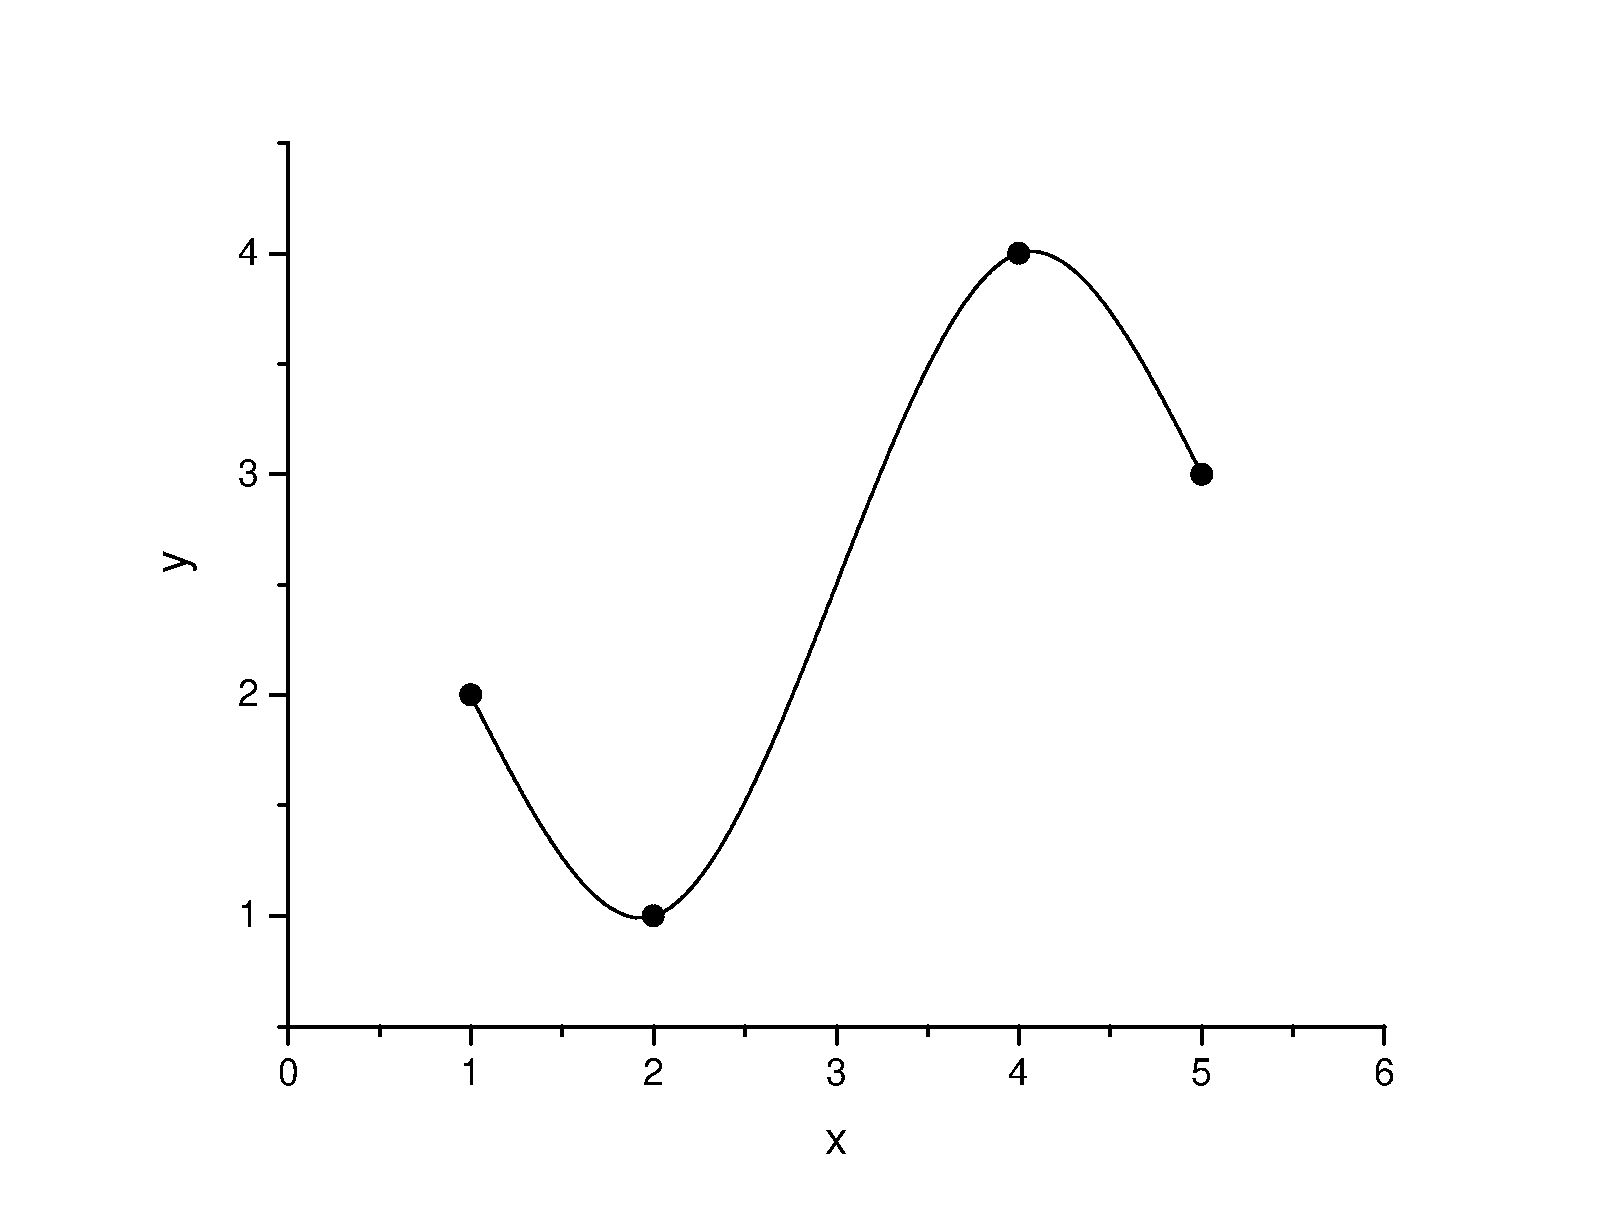
\includegraphics[width=5.5cm]{pulse_preprocess/spline2}
    }
    \caption{\label{fig:spline}经过4点的线性样条插值与三次样条插值对比}
\end{figure}

多项值插值与样条插值是插值最常用的两种算法\cite{Timothy2018,Carl2008}。多项式插值给出满足所有原始数据点的单一公式,由于此过程中仅涉及浮点数加法与乘法,可以很方便的在PC及嵌入式设备上实现,因而得到广泛应用。
而样条插值则使用多个公式来通过所有数据点,其中每个公式均为低阶多项式。三次样条插值是样条插值在工业领域应用最广泛的算法之一,可以得到光滑的拟合插值曲线。
具体而言,对原始数据点$(x_1,y_1),(x_1,y_1),\cdots,(x_n,y_n)$,三次样条的插值曲线$S(x)$在每两个数据分段区间$[x_i,x_{i+1}]$内均使用三阶多项式
\begin{equation}
    \label{equ:spline}
    S_{i}=y_{i}+b_{i}(x-x_{i})+c_{i}{(x-x_{i})}^2+d_{i}{(x-x_{i})}^3
\end{equation}
并保证每两个多项式在端点(即原始数据点)处不仅数值相等,相应的斜率与曲率均相等,即
\begin{equation}
    \label{equ:cubiccha}
    \left \{
    \begin{aligned}
        S_{i}(x_{i})&=y_i,&\text{i=1,$\cdots$,n-1}\\
        S_{i}(x_{i+1})&=y_{i+1},&\text{i=1,$\cdots$,n-1}\\
        S_{i}^{'}(x_{i-1})&=S_{i}^{'}(x_{i}),&\text{i=2,$\cdots$,n-1} \\
        S_{i}^{''}(x_{i-1})&=S_{i}^{''}(x_{i}),&\text{i=2,$\cdots$,n-1}
    \end{aligned}
    \right.
\end{equation}
使用微积分的定义,将\autoref{equ:spline}代入\autoref{equ:cubiccha}化简整理后,可以得到包含$3n-5$个独立方程的方程组。另一方面,由于每个局部$S_i$中有三个未知参数,一共有$3n-3$个待解参数,则此时由线性代数相关知识可知,该方程组有无穷多组解。
即此时可以构造处无穷多条通过所有数据点$(x_i,y_i)$的样条曲线。因此,需要添加额外的方程对样条曲线进行约束,一般的约束条件都是对样条左右端点处进行限定 ,常见的附加边界条件如\autoref{tab:splinekind}所示\cite{Timothy2018}。
\begin{table}[htbp]
    \centering
    \caption{\label{tab:splinekind}几种常见的三次样条端点条件}
    \begin{tabularx}{\linewidth}{X<{\centering}X<{\centering}}
        \toprule 
        \textbf{样条种类}&\textbf{端点条件}\\
        \midrule 
        自然三次样条&
        $
            S_{1}^{''}(x_{1})=0,
            S_{n-1}^{''}(x_{n})=0
        $
        \\
        曲率调整三次样条&
        $\left \{
        \begin{aligned}
            &S_{1}^{''}(x_{1})=v_1,&v_{1}\neq0\\
            &S_{n-1}^{''}(x_{n})=v_n,&v_{n}\neq0
        \end{aligned}
        \right.
        $
        \\
        钳制三次样条&
        $\left \{
        \begin{aligned}
            &S_{1}^{'}(x_{1})=v_1,&v_{1}\neq0\\
            &S_{n-1}^{'}(x_{n})=v_n,&v_{n}\neq0
        \end{aligned}
        \right.
        $
        \\
        抛物线端点三次样条&
        $
            d_1=0,d_{n-1}=0
        $
        \\
        非纽结三次样条&
        $
            d_1=d_2, d_{n-2}=d_{n-1}
        $
        \\
        \bottomrule
    \end{tabularx}
\end{table}

在补充\autoref{tab:splinekind}中的两个端点条件公式后,即可完成上述方程组求解,从而确定唯一的三次样条插值曲线。本研究中三次样条算法基于自然边界条件对PPG信号进行均匀插值\cite{ttk2021},使信号采样率被提高至2000$Hz$。
\subsection{数据标准化}
在上述各项预处理过程完成后,此时得到的PPG数据在波形幅值上仍然有很大的个体差异,即使对同一被试对象,其波形在幅值上也会有一定的波动。为消除个体差异对特定波形特征计算的影响,需要对脉搏波信号进行归一化处理。

时间标准化与幅值标准化是PPG标准化两类常见的方式\cite{mmt}。时间标准化的基本原理是将PPG信号进行分组并计算每组信号的平均心动周期,随后对每组内的PPG信号进行时间尺度上的缩放,使最终的总平均心动周期保持一致。
由于不同个体的时间尺度上的缩放比例不一致,很容易导致PPG信号波形发生畸变失真,严重影响后续特征计算。故本研究采取了幅值标准化的处理方式对PPG信号进行处理。

由第二章PPG信号光学采集的基本原理可知,PPG信号的波形幅值对不同个体而言并无实际的生理意义,这保证了对PPG信号幅值标准化的合理性。与去除基线漂移过程类似,对待处理的特定PPG波形内所有采样点进行一次线性变换即可完成处理。
为使后续特征计算各项数值不会出现大量的小数,本研究没有采用最常见的归一化处理,而是将单个波形内所有数据点按同一尺度缩放映射到$[0,1000]$区间内。
另一方面,对于同一被试的不同PPG波形而言,其幅值的相对高低变化可能蕴含了一定的生理信息。因此,在标准化过程中,所有波形的标准化系数即缩放比例也同时被保存记录下来。

\section{脉搏波的描述}
绪论中已经介绍过,PPG信号本身蕴含着丰富的血液动力学信息,其形态、强度、速率、节律等特征可以反映心脏的功能与状态,也可以反映出各级动脉及分支中血管壁弹性、血管阻力、血液黏度等信息,是评价人体心血管系统生理病理状态的重要依据\cite{PPGYY}。
换言之,脉搏波信号携带了能够表征人体心血管系统生理病理状态的全部信息,这些信息蕴藏在了PPG波形的变化之中。因此,用何种方式描述、获取、挖掘这些信息,是基于脉搏波的分析工作能够开展的前置条件。
\begin{figure}[htbp]
    \centering
    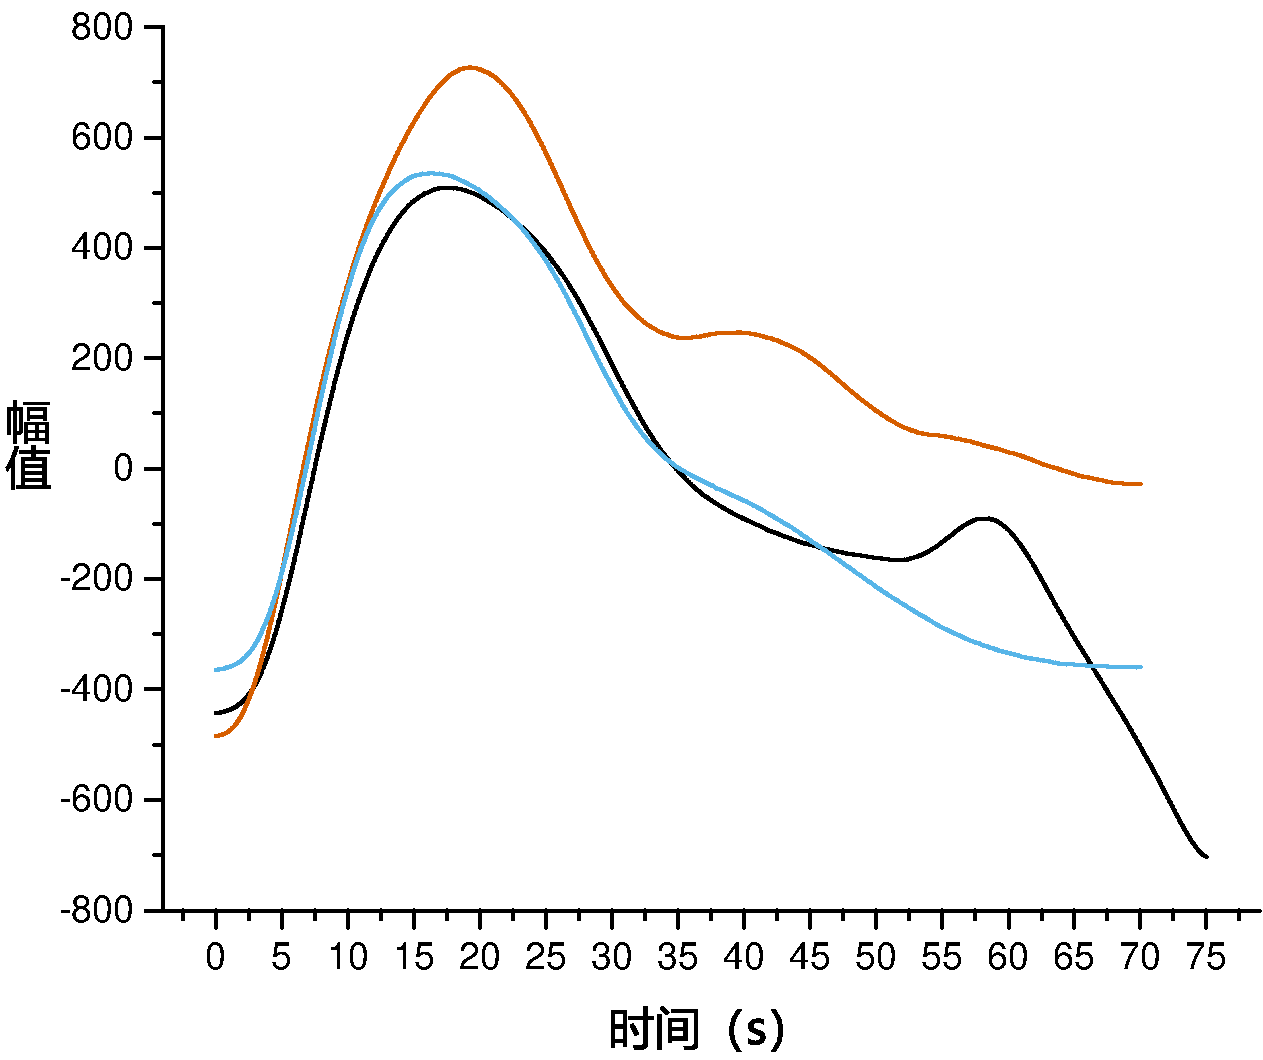
\includegraphics[width=.6\linewidth]{pulse_preprocess/pulsecontrast}
    \caption[同一名被试PPG信号三段波形对比]{\label{fig:pulsecontrast}同一名被试PPG信号三段波形对比。波形按起点时间对齐,此外无任何其他预处理操作。可以看到三段波形在重搏的显著程度、时长、幅值等方面均有所差异。}
\end{figure}
\subsection{描述的本质}
通信工程中认为,信息是事物运动状态或存在方式的不确定性描述,是通信的内涵;消息是能够被人体感觉器官所感知的物理现象,是信息的外在表现形式;信号则是消息的物理表现形式,是消息的载体\cite{Shannon1948,Liu2019,Zhao2017}。
目前较为常见的完整通讯系统模型如\autoref{fig:communication}所示。其中,信源是产生消息的源头,是通信的起点。信道是信息的传输媒介,是对实际传输过程的抽象,由于信息的传输过程中会难以避免的引入噪声与干扰,
通信工程常将系统各部分所受到的干扰与噪声折合成信道干扰。\autoref{fig:communication}中的编码过程与解码过程则是为保证传输质量与通讯稳定而对消息符号按照预设的规则进行编码与解码工作。
信宿则是信息传输的目的地,也是接收消息的对象,是本次通信的终点\cite{Zhao2017}。
\begin{figure}[htbp]
    \centering
    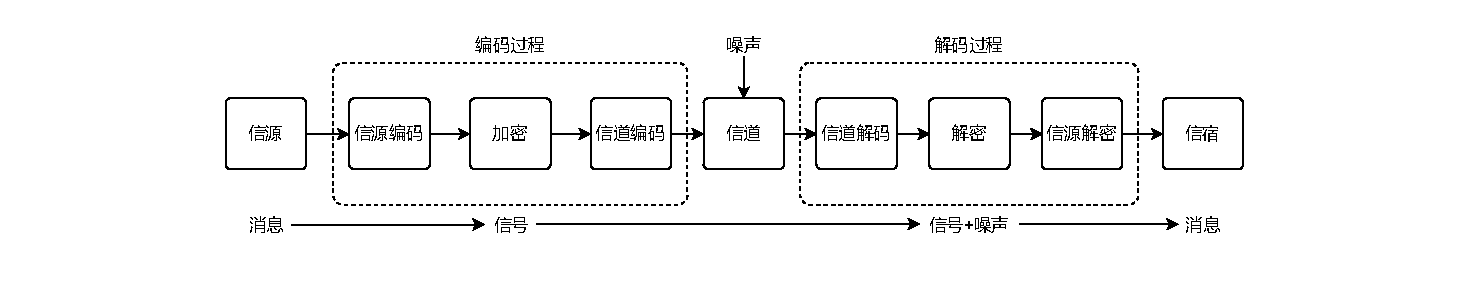
\includegraphics[width=\linewidth]{pulse_preprocess/communication}
    \caption[通信系统模型框图]{\label{fig:communication}通信系统模型框图\cite{Zhao2017,Liu2019}}
\end{figure}

若从通信原理的角度来看待信号分析的一般过程,那么所有基于人体电生理信号的相关研究均可以抽象地看成特定生理信息从人体或人体某一器官到研究学者、临床医生等之间的信息传输问题,如\autoref{fig:ppgcommunication}所示。
以本研究涉及的脉搏波PPG信号为例,那么搏动不止的心脏显然是这一通讯系统的信源,人体内各脏器系统、组织等可以看成是一个复杂的黑箱编码系统(此部分参见第二章脉搏波产生原理的脉搏波参数模型与非参数模型相关内容)。人体表面丰富的毛细血管则是
该通讯过程中的信道,若因PE等疾病引起了人体毛细血管等系统的生理性变化可以折合成对信道的干扰噪声。而PPG信号本身则是反映信源心脏功能与信道基本特性的消息载体。\textbf{在此基础上,脉搏波的描述过程即可视为在编码规则不明确(黑箱模型)的前提
下对携带上述生理信息的信号进行译码解码的过程。}
\begin{figure}[htbp]
    \centering
    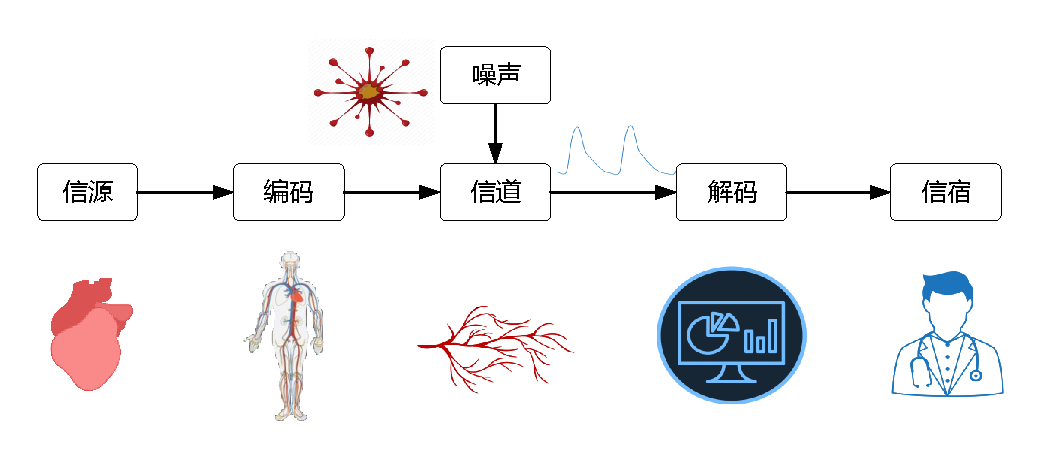
\includegraphics[width=.8\linewidth]{pulse_preprocess/ppgcommunication}
    \caption{\label{fig:ppgcommunication}以通讯工程的视角看待脉搏波的分析过程}
\end{figure}

另一方面,PPG信号常以一个数字序列表示在一定的采样时间该信号的所有采样值,其序列的长度与信号采样率成正比,一般在100$Hz$以上。而不论是类似“该波形周期较长”、“该波形重播波潮波不明显”等自然语言描述(经过数字标签化处理后),
还是以“下降支时长为0.43s”、“该波形波峰幅值为1351”等绝对量化的数值描述,都是以较少的数值去完成PPG信号的描述与评估过程。显然,\textbf{上述PPG信号的数字量化过程亦是一个降维处理过程,其本质仍是信息压缩。}
因此,此前诸多学者提出的多项PPG特征参数就是从不同侧面对原始数据进行数字量化与降维处理的过程。

\subsection{常见的脉搏波时域特征}
通常而言,对信号进行分析可以采取时域-频域联合分析方法。由于脉搏波本身频域带宽窄,且数据采集实验得到的数据波形较为简单、干扰少、整体质量较高,故本研究主要从\textbf{时域角度}对脉搏波进行特征提取与描述工作。
本小节将前人提出的脉搏波时域特征进行了汇总整理,将PPG相关描述特征按计算时是否基于完整PPG波形分为基于波形与基于时间窗等两大类。其中,基于时间窗的特征又可进一步细分为基于5s、10s等固定窗长与不定窗长等两大类。
特别地,本小节也对已在子痫前期的相关研究中得到应用的脉搏波(含压力脉搏波)特征参数进行了详细说明。

一、基于波形的时域特征

在诸多PPG波形形态学特征参数中,时间类参数、幅度类参数与面积类参数往往定义清晰明了、意义明确易于理解、且易与脉搏波产生原理过程联系起来,从而具有一定的生理学意义。
因此,这些参数在基于PPG的各类研究中得到了最广泛的应用\cite{cwl,mmt}。除这三类参数外,斜率类参数也在描述脉搏波形态特征领域占有一席之地。
最后,在信号分析领域得到广泛使用的通用无量纲参数与高阶统计参数也可在一定程度上反应PPG信号特征。
以下是各类参数的具体介绍。

1. 时间类特征参数

时间类特征参数描述了PPG波形中某些特殊点之间的时长值或多个这样时长之间的比例关系。脉搏传导时间(Pulse Transit Time,PTT)则是其中最有代表性的时间类参数之一。
如\autoref{fig:ri}所示,PTT是对脉搏波主波峰与重博波波峰或反射波导致的拐点之间的时间间隔的量化描述\cite{Brumfield2005,Su2014}。PTT在基于PPG的各类研究中得到了广泛应用。
\begin{figure}[htbp]
    \centering
    \subfigure[\label{fig:ri1}重博波明显的PPG波形]{
    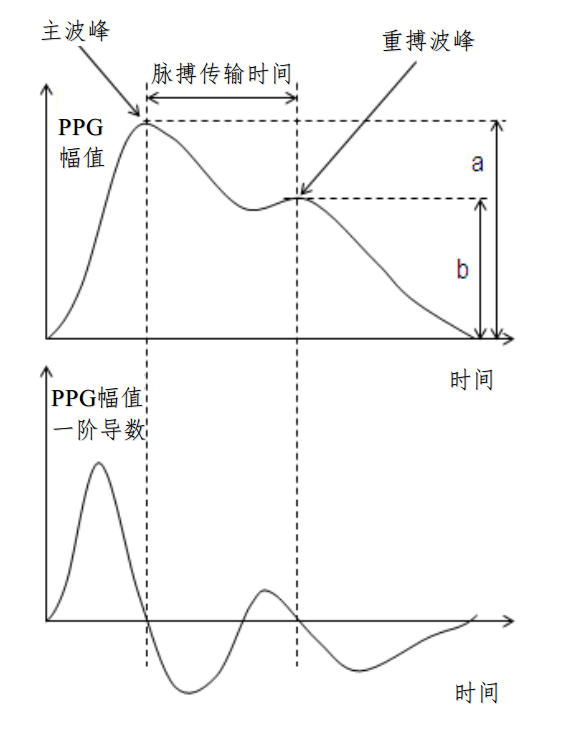
\includegraphics[width=5.5cm]{pulse_preprocess/ri1}
    }
    \quad
    \subfigure[\label{fig:ri2}重博波不明显的PPG波形]{
    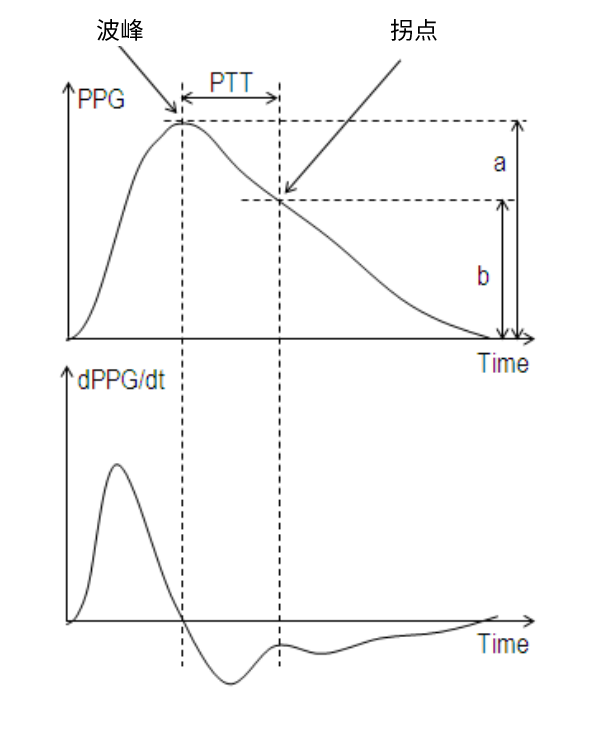
\includegraphics[width=5.5cm]{pulse_preprocess/ri2}
    }
    \caption[PTT及RI计算原理示意]{\label{fig:ri}PTT及RI计算原理示意\cite{Su2014}}
\end{figure}

除PTT外,时间类特征参数还包含脉搏波脉动周期、上升支间期、下降支间期等。2016年,王梦婷提出了一种描述动脉内高压力水平维持的时间参数,并在此基础上归一化处理后得到了多项衍生参数,
包含动脉高压力持续时间、血管硬度指数、心肌收缩系数及心博出系数等\cite{mmt}。
2018年,陈婉琳等人基于斜率极值提出了上升支最大斜率间期、下降支最小斜率间期等参数\cite{cwl}。以上参数的定义参见\autoref{fig:timefeature}及\autoref{tab:timefeature}所示。
\begin{figure}[htbp]
    \centering
    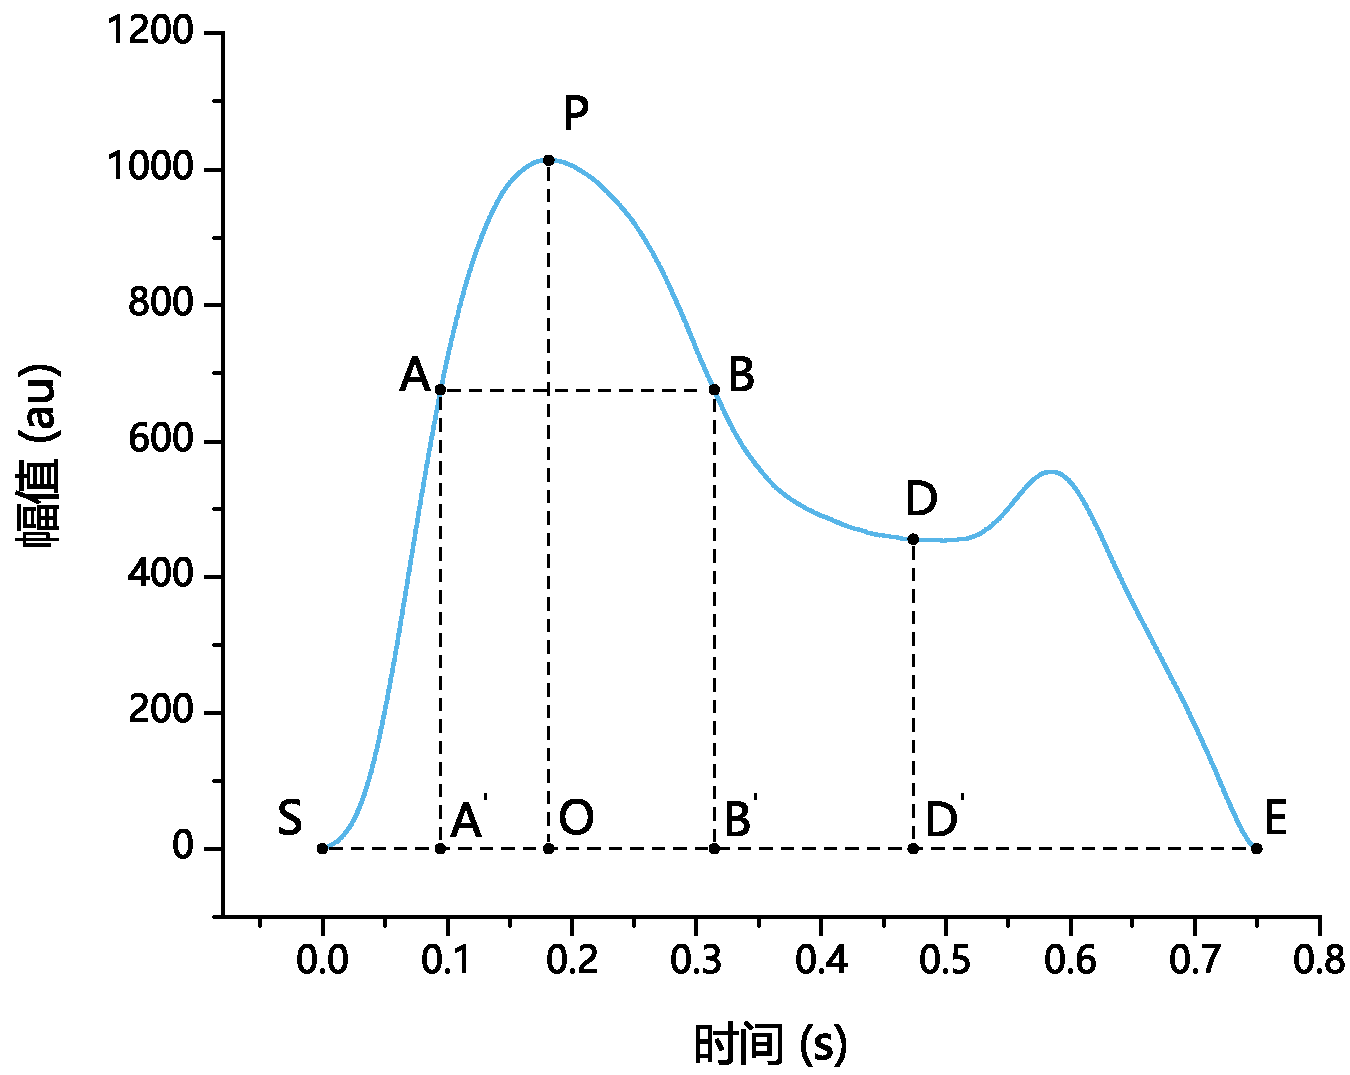
\includegraphics[width=.6\linewidth]{pulse_preprocess/timefeature}
    \caption[PPG时间及幅值类参数示意]{\label{fig:timefeature}PPG时间及幅值类参数示意。其中,AA'的幅值为主波峰值的2/3,D点为降中峡。}
\end{figure}
\begin{table}[h]
    \centering
    \caption{\label{tab:timefeature}常见PPG时间类参数定义}
    \begin{tabularx}{\linewidth}{cX<{\centering}c}
    \toprule
    \textbf{参数} & \textbf{物理意义} & \textbf{表达式} \\
    \midrule
    脉动周期      &  相邻两个波谷之间的时间间隔         &  $SE$\\
    上升支间期      &  从波形起点(波谷)至主波峰之间的时间间隔         &  $SO$\\
    下降支间期      &  从主波峰至波形终点(波谷)之间的时间间隔        &  $OE$\\
    动脉高压力持续时间    &  主波维持在峰值幅值2/3高度的时间间隔         &    $A'B'$   \\
    血管硬度指数    &  动脉高压力持续时间与脉动周期的比值         &   $\frac{A'B'}{SE}$    \\
    心肌收缩系数    &  上升支间期与脉动周期的比值         &  $\frac{SO}{SE}$    \\
    心搏出系数      &   从波峰至降中峡的时间间隔与脉动周期的比值       &   $\frac{OB'}{SE}$\\
    上升支最大斜率间期      &   上升支波谷与上升支斜率最大点之间的时间间隔      &   /    \\
    下降支最大斜率间期      &   下降支斜率最小点与下降支波谷之间的时间间隔      &    /  \\
    \bottomrule
    \end{tabularx}
\end{table}

2. 幅值类特征参数

幅值类特征参数描述了PPG波形中某个时刻的幅值高度或多个时刻幅值高度之间的比例关系。在各项研究中得到普遍应用的脉搏波增强指数(Augmentation Index,AIX)、反射指数(Reflection Index,RI)及K值等
均属于幅值类参数。

AIX指心脏收缩期早期与晚期拐点之间的差值与峰值之比,计算的关键需要先找到表征脉搏波反射波上升冲程(up-stroke)的拐点$P1$,如\autoref{fig:aix}所示\cite{Su2014}。
\begin{equation}
    \label{equ:aix}
    AIX = \pm \frac{\Delta P}{PP}
\end{equation}
特别地,\autoref{equ:character}中$\pm$的取值视拐点$P1$与峰值点的相对位置而定。当拐点在脉搏波波峰点左侧时,AIX符号取正,表示主波峰是经过叠加得到的,如图\autoref{fig:aix1}所示;反之,
当拐点在脉搏波波峰点右侧时,AIX符号取负,表明主波峰未得到“增强”,如图\autoref{fig:aix2}所示。
\begin{figure}[htbp]
    \centering
    \subfigure[\label{fig:aix1}拐点在波峰左侧]{
    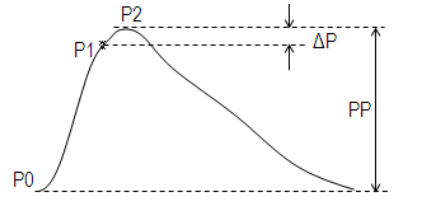
\includegraphics[width=5.5cm]{pulse_preprocess/aix1}
    }
    \quad
    \subfigure[\label{fig:aix2}拐点在波峰右侧]{
    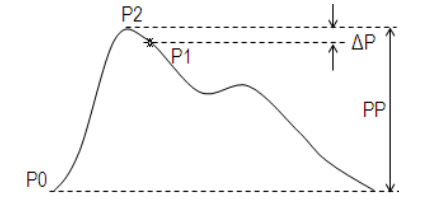
\includegraphics[width=5.5cm]{pulse_preprocess/aix2}
    }
    \caption[AIX计算原理示意]{\label{fig:aix}AIX计算原理示意\cite{Su2014}}
\end{figure}

RI是由脉搏波舒张峰值或拐点处幅值与收缩谷值之比计算得到的,如\autoref{fig:ri}所示\cite{Su2014,Elgendi2012}
\begin{equation}
    \label{equ:ri}
    RI = \frac{b}{a} \cdot 100\%
\end{equation}

K值是另一种在临床得到广泛应用的基于脉搏波面积变化的形态学特征无量纲参数,最早由罗志昌等人提出\cite{Luo1988,PPGYY}
\begin{equation}
    \label{equ:ppgk}
    K=\frac{P_m-P_d}{P_s-P_d}
\end{equation}
其中,$P_m=\frac{1}{T}\int_{0}^{T}P(t)dt$为一个心动周期内脉搏压力$P(t)$的平均值,$P_s$与$P_d$分别为收缩压与舒张压。罗志昌等人的研究表明,K值依赖于脉搏波的波形动态变化,
同时能够在很大程度上反应血管外周阻力与血管壁硬化程度等生理因素的变化。
\begin{figure}[htbp]
    \centering
    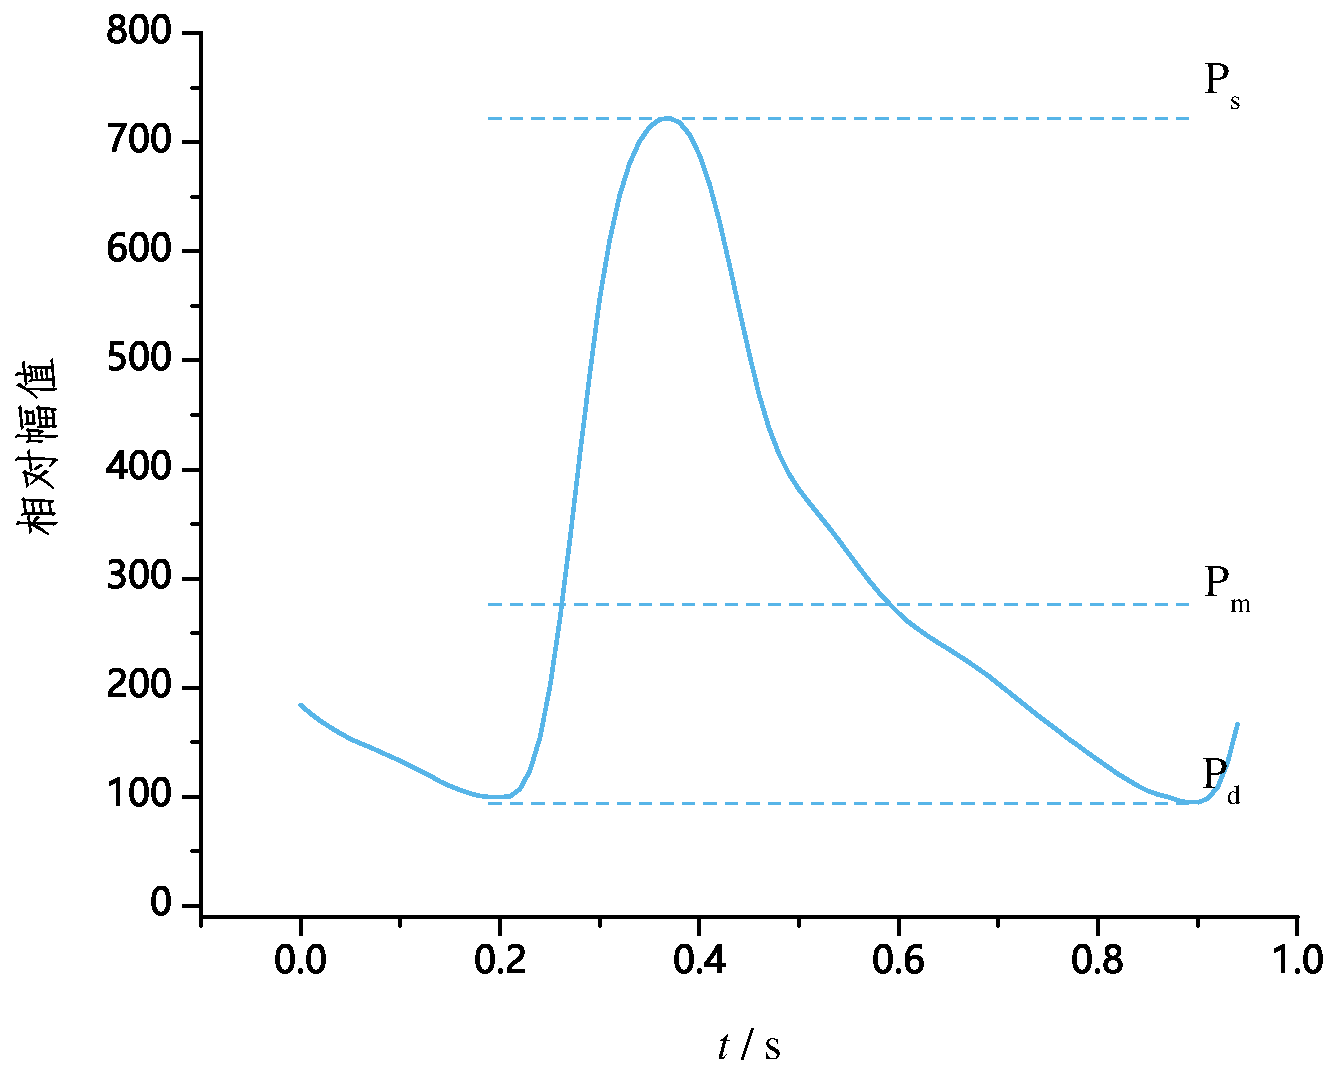
\includegraphics[width=.55\linewidth]{pulse_preprocess/k}
    \caption{\label{fig:k}K值的计算原理示意}
\end{figure}

除上述参数外,幅值类特征参数还包括脉搏波波峰幅值、波谷幅值差值、降中峡幅值及外周阻力系数等\cite{cwl,mmt}。这些参数的具体定义参见\autoref{fig:timefeature}及\autoref{tab:heightfeature}所示。
\begin{table}[htbp]
    \centering
    \caption{\label{tab:heightfeature}常见PPG幅值类参数定义}
    \begin{tabularx}{\linewidth}{cX<{\centering}c}
    \toprule
    \textbf{参数} & \textbf{物理意义} & \textbf{表达式} \\
    \midrule
    波峰幅值      &  主波峰幅值         &  $OP$\\
    波谷幅值差值      &  相邻波谷之间的幅值之差         &  /\\
    降中峡幅值      &  降中峡至基线幅值         &  $DD'$\\
    外周阻力系数      &  降中峡幅值与主波峰幅值之比         &  $\frac{DD'}{OP}$\\
    \bottomrule
    \end{tabularx}
\end{table}

3. 面积类特征参数

面积类参数计算依赖与脉搏波波形与基线所形成的面积,主要通过按时间方向对PPG波形曲线积分完成计算过程。
面积类参数可以看成是血管在一段时间内的血液容积的映射。
王梦婷在其研究中指出\cite{mmt},PPG上升支主要受心脏射血量与血压脉动影响,下降支主要受外周阻力影响。其中,上升支随心脏射血量增加愈益陡峭,射血时间越短,
其形态图像越向左上方凸出;而当外周阻力增加时,会导致动脉血管壁弹性下降,下降支波形向上方凸出。

常见的面积类特征参数包括上升支面积、下降支面积、
全周期面积、上升支面积比、下降支面积比、全周期面积比及(下降支)面积差值比(Area Difference Ratio,ADR)\cite{Feng2018}等。
以上参数的具体定义参见\autoref{fig:areafeature}及\autoref{tab:areafeature}。
\begin{figure}[htbp]
    \centering
    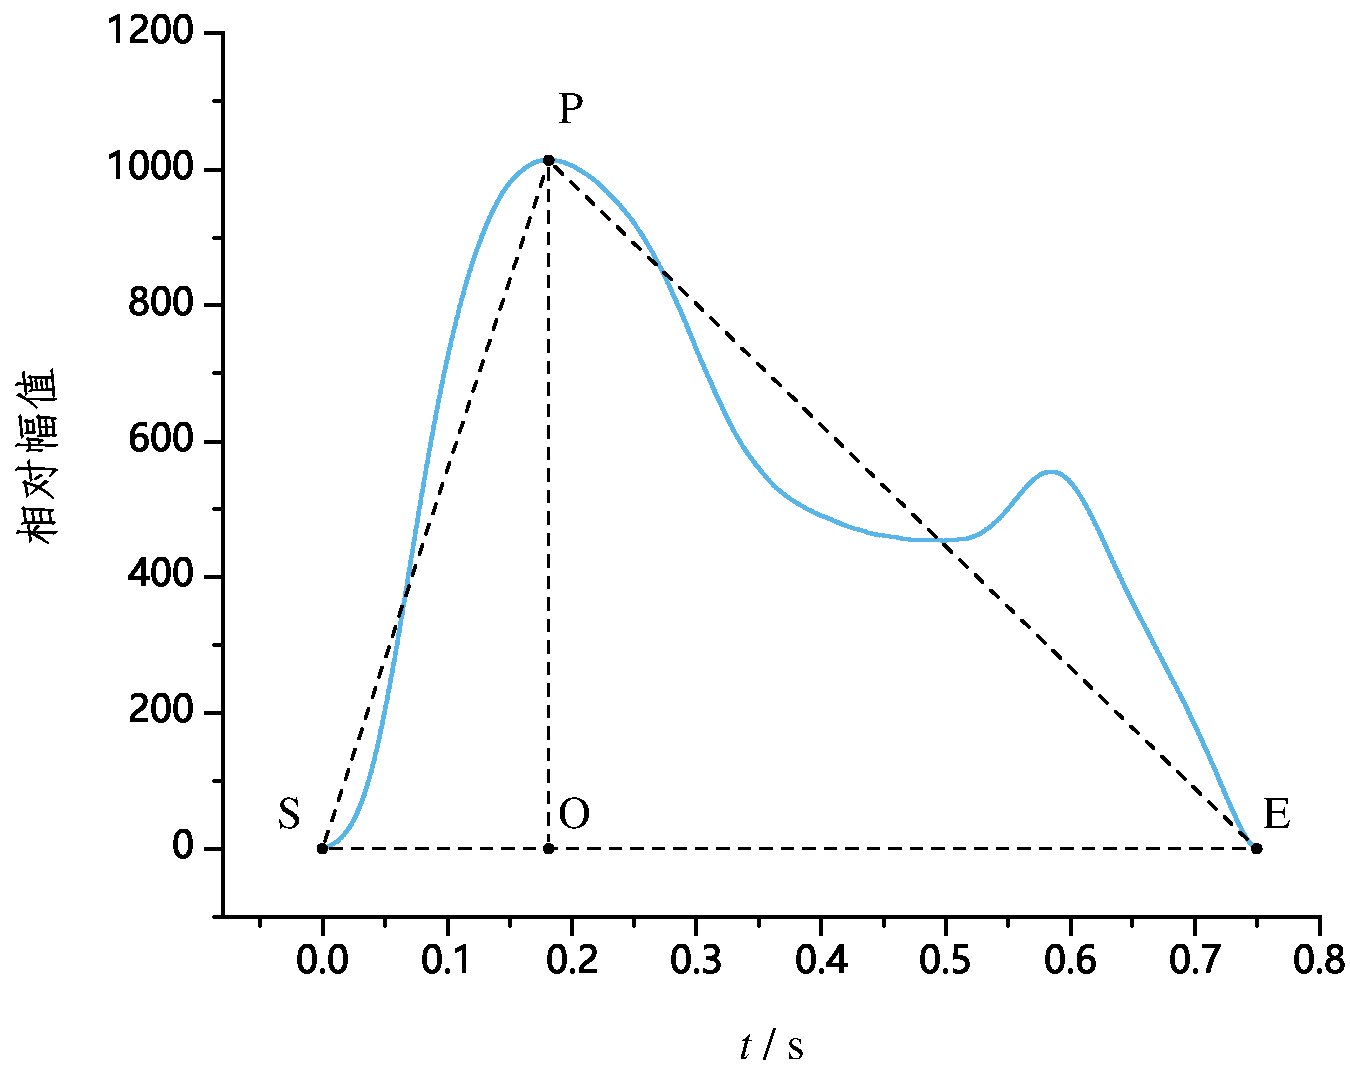
\includegraphics[width=.6\linewidth]{pulse_preprocess/areafeature}
    \caption{\label{fig:areafeature}PPG面积及斜率类参数示意}
\end{figure}

\begin{center}
    % \zihao{5}
	\begin{longtable}{m{3.5cm}<{\centering}m{6.5cm}<{\centering}m{4.5cm}<{\centering}}
		\caption{PPG面积类参数示意}\\
		\label{tab:areafeature}\\
        \toprule
        \textbf{参数} & \textbf{物理意义} & \textbf{表达式} \\
        \midrule
        \endfirsthead
        \caption[]{(续)}\\
        \toprule
        \textbf{参数} & \textbf{物理意义} & \textbf{表达式} \\
        \midrule
        \endhead 
        \midrule
        \endfoot
        \bottomrule
        \endlastfoot
        上升支面积      &  从波形起点至峰值点对波形曲线积分所得面积值         &  $S_r=\int_{T_S}^{T_P}P(t)dt$\\
        下降支面积      &  从波形峰值点至终点对波形曲线积分所得面积值         &  $S_f=\int_{T_P}^{T_E}P(t)dt$\\
        全周期面积      &  脉搏波波形在一个完整周期内的积分所得面积值         &  $S_t=\int_{T_S}^{T_E}P(t)dt$\\
        上升支面积比    &  上升支面积与$\triangle OPS$面积之比         &   $R_r=\frac{S_r}{S_{\triangle OPS}}$    \\
        下降支面积比    &  下降支面积与$\triangle OPE$面积之比        &   $R_f=\frac{S_f}{S_{\triangle OPE}}$    \\
        全周期面积比    &  全周期面积与$\triangle SPE$面积之比         &   $R_t=\frac{S_t}{S_{\triangle SPE}}$    \\
        下降支面积差值比&  下降支面积和$\triangle OPE$面积之差与$\triangle OPE$面积之比        &    $\Delta R_f=\frac{S_{\triangle OPE}-S_f}{S_{\triangle OPE}}=1-R_f$\\
	\end{longtable}
\end{center}

值得一提的是,Feng等人已经将ADR应用于子痫前期的研究中,其研究结果显示患有PE的孕妇与正常孕妇在PPG信号的ADR参数上具有统计意义上的显著差异(0.752 VS 0.723,P<0.01)\cite{Feng2018}。

另外需要注意的是,从\autoref{tab:areafeature}中的参数定义不难发现,ADR与下降支面积比完全线形相关,两者之间满足
\begin{equation}
    \label{equ:adr}
    ADR = 1-R_f
\end{equation}
此外,王选在其研究中也证明了全周期面积比与幅值类参数K值完全线性相关\cite{Wang2012}
\begin{equation}
    \label{equ:kandart}
    R_t=\frac{S_t}{S_{\triangle SPE}}=\frac{\int_{0}^{T}P(t)dt}{\frac{1}{2}P_sT}=\frac{2\cdot P_mT}{P_sT}=2\cdot K
\end{equation}
因此,若需要使用这两组参数对PPG进行描述时,只需视情况分别从每组中选取一个即可。

4. 斜率类特征参数

斜率类参数是对PPG波形在一段时间内幅值的上升/下降速率的快慢的量化描述,反应了血液容积在这段时间内的平均流速。

光电容积斜率指数(photoplethysmography slope index,PSI)是斜率类参数中比较有代表性的一种\cite{Chen2019}。其计算的基本思想是将PPG波形分段后再描述各段之间的幅值变化,
如\autoref{fig:psi}所示。
\begin{figure}[htbp]
    \centering
    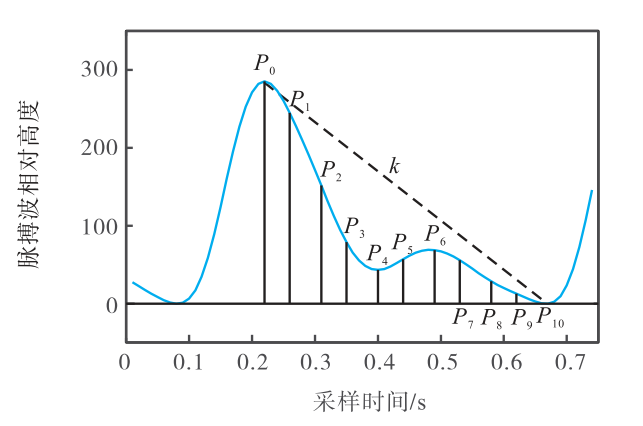
\includegraphics[width=.6\linewidth]{pulse_preprocess/psi}
    \caption[PSI计算原理示意]{\label{fig:psi}PSI计算原理示意\cite{Chen2019}}
\end{figure}
值得一提的是,陈婉琳等人的研究发现PSI可以在一定程度上对PE患者进行识别\cite{Chen2019}。

此外,常见的斜率参数还包括上升支平均斜率、上升支最大斜率、下降支平均斜率、下降支最大斜率等。这些参数的具体定义参见\autoref{fig:areafeature}及\autoref{tab:slopefeature}所示。
\begin{table}[htbp]
    \centering
    \caption{\label{tab:slopefeature}常见PPG斜率类参数定义}
    \begin{tabularx}{\linewidth}{cX<{\centering}c}
    \toprule
    \textbf{参数} & \textbf{物理意义} & \textbf{表达式} \\
    \midrule
    上升支平均斜率      &  主波峰值与上升支时间之比         &  $\frac{OP}{SO}$\\
    下降支平均斜率      &  主波峰值与下降支时间之比         &  $-\frac{OP}{OE}$\\
    上升支最大斜率      &           &  /\\
    下降支最小斜率      &           &   /    \\
    \bottomrule
    \end{tabularx}
\end{table}

5. 通用无量纲参数与高阶统计量

无量纲参数(non-dimensional parameter)是指不使用计量学中基本单位及导出单位进行衡量的参数,该类参数通常以比值的形式出现。故严格意义来说,前文中介绍的参数中所有比值类参数均可划归至无量纲参数中。
无量纲参数作为信号时域分析重要参考指标,在机械控制、石油石化、电信电子、地球物理、故障诊断、信号处理等领域有着广泛的应用\cite{Jardine2006,Guo2014,Tu2013,Mendel1991}。本研究中使用了常见的峰值因子(crest factor)、
脉冲因子(impulse factor)、裕度因子(clearance factor)及波形因子(form factor)等指标对脉搏波信号进行评估,相关参数的基本定义如\autoref{tab:ndp}所示。

高阶统计量(High Order Statitics,HOS)是指非传统的二阶统计量(如时域相关函数、频域功率谱密度等),通常是三阶或三阶以上的统计量\cite{Zhang2002,Tu2013}。高阶统计量是研究分析非线形、非因果、非最小相位系统和非高斯、非平稳、非加性噪声的重要分析工具。
本研究使用了高阶统计量中表示分布的峭度因子(kurtosis factor)与偏度(skewness)对PPG信号进行了评估,两者的基本定义参见\autoref{tab:ndp}。
\begin{table}[htbp]
    \centering
    \caption{\label{tab:ndp}常见的无量纲参数及高阶统计量}
    \begin{tabularx}{\linewidth}{cX<{\centering}c}
        \toprule
        \textbf{参数}&\textbf{物理(统计)意义}&\textbf{定义方程}\\
        \midrule
        峰值因子&信号峰值与信号有效值(均方根值)的比值& $C=\frac{X_{peak}}{X_{RMS}}$      \\
        脉冲因子&信号峰值与信号整流值(绝对值的平均值)的比值&$I=\frac{X_{peak}}{|\bar{X}|}$      \\
        裕度因子&信号峰值与信号方根幅值的比值&$C_e=\frac{X_{peak}}{X_R}$       \\
        波形因子&信号有效值与信号整流值的比值&$S_f=\frac{X_{RMS}}{|\bar{X}|}$      \\
        峭度因子&信号四阶中心矩和信号标准差的四次方的比值&$K_4=\frac{E[(X-\mu)^4]}{\sigma^4}$      \\
        偏度&信号三阶中心矩和信号标准差的三次方的比值&$K_3=\frac{E[(X-\mu)^3]}{\sigma^3}$      \\
        \bottomrule
    \end{tabularx}
\end{table}
\begin{figure}[htbp]
    \centering
    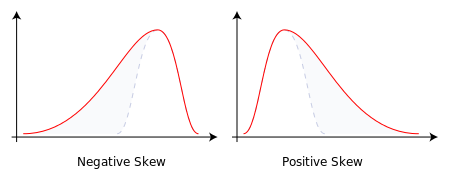
\includegraphics[width=.6\linewidth]{pulse_preprocess/skew}
    \caption{\label{fig:skew}峭度因子与偏度示意}
\end{figure}

从\autoref{tab:ndp}可以发现,峰值因子、脉冲因子、裕度因子具有相似的物理定义,均是信号峰值与原始信号的某一统计量均值进行比较。由数字信号处理的原理可知,均值计算可以看成是一个简单的低通滤波模型,
对突变的脉冲信号有较好的抑制作用。因而,这三个非量纲参数对脉冲冲击导致的峰值变化比较敏感。
而波形因子则是两个统计量均值的比值,对脉冲信号的敏感性不高。另一方面,高阶统计量峭度因子和偏度反应的是原始信号的分布特性,如\autoref{fig:skew}所示。峭度因子常在信号处理中作为高斯信号与非高斯信号的划分标准,高斯信号的峭度因子为3。
偏度则主要反应信号的左右对称性,完全对称的信号其偏度为0。

二、基于时间窗的时域特征

与先定位好具体的PPG波形再进行计算的PPG时域参数不同,另一种描述PPG波形的思路则以时间窗为单位,关注时间窗内的原始信号的整体统计特征再进行具体参数的计算,而时间窗的长度一般也从数秒至数十秒不等。

收缩压变异性(Systolic pressure variation,SPV)与脉压变异性(pulse pressure variation,PPV)则是两个有代表性的时间窗类特征,如\autoref{fig:spv}所示\cite{GE2021,Michard1999,Perel1987,Michard2005}。
人体的呼吸作用会导致胸腔内血压出现变化,使得血容量不同的人群在脉搏波的幅值存在一定的差异性。
在对人体体液状况进行评估时,常使用动脉压变异性(arterial pressure variation,APV)的方法。SPV与PPV则是进行APV分析时的两个具体指标,其定义分别为\cite{GE2021}:
\begin{equation}
    \label{equ:spv}
    SPV=SBP_{max}-SBP_{min}
\end{equation}
\begin{equation}
    \label{equ:ppv}
    PPV=\frac{PP_{max}-PP_{min}}{\frac{PP_{max}+PP_{min}}{2}}\cdot 100\%=\frac{PP_{max}-PP_{min}}{PP_{max}+PP_{min}}\cdot 200\%
\end{equation}
其中,$SBP_{max}$与$SBP_{min}$分别代表时间窗内收缩压的最大值和最小值;$PP_{max}$与$PP_{min}$代表时间窗内脉压最大值和最小值;时间窗的宽度与步进值均为5s,即每5s完成一次两个参数的计算工作。
\begin{figure}[htbp]
    \centering
    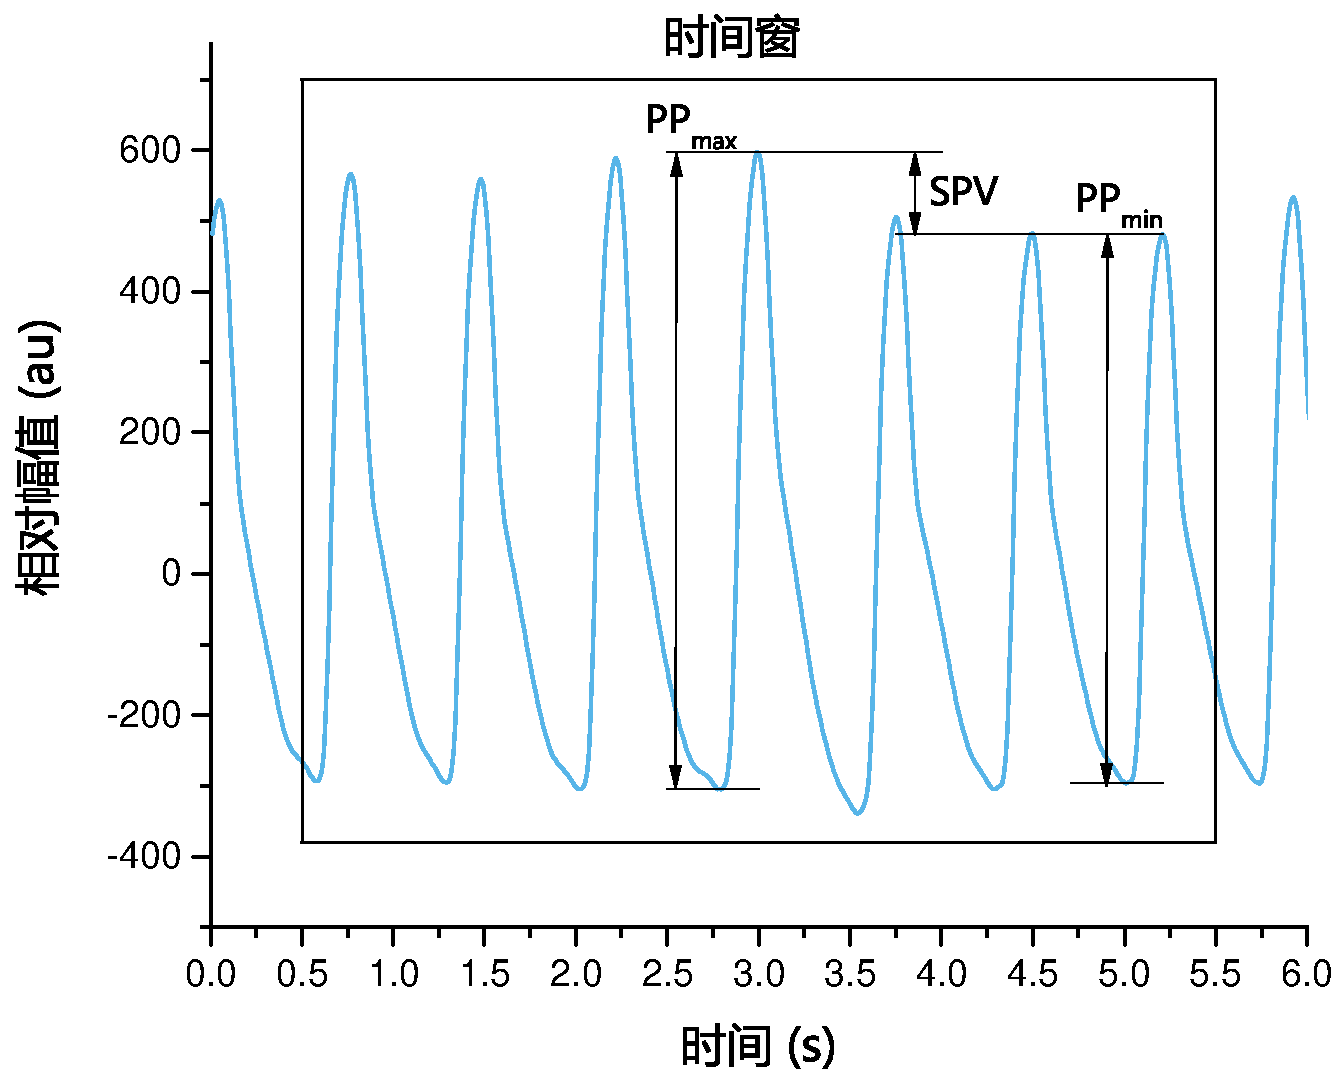
\includegraphics[width=.6\linewidth]{pulse_preprocess/spv}
    \caption{\label{fig:spv}SPV与PPV示意}
\end{figure}

三、其他特征

除上述特征参数外,在PPG的其他研究领域还有一些较为知名的特征参数,大动脉僵硬指数(stiffness index,SI)与脉搏波波形速度(Pulse Wave Velocity,PWV)就是其中最为典型的代表。

SI被定义为是被试身高$h$与脉搏波的主波峰值降中峡的时间间隔$\Delta T$的比值\cite{Elgendi2012,Millasseau2002,Brumfield2005},即
\begin{equation}
    \label{equ:si}
    SI = \frac{h}{\Delta T}
\end{equation}
Millasseau等人的研究表明随着大动脉硬度增加、主动脉和大动脉中压力波的脉搏波速度增加,
收缩和舒张峰值之间的时间延迟也会随着年龄的增长而减少,导致SI也会随着年龄增长而增长,如\autoref{fig:si}所示\cite{Elgendi2012,Millasseau2002,Brumfield2005}。
\begin{figure}[htbp]
    \centering
    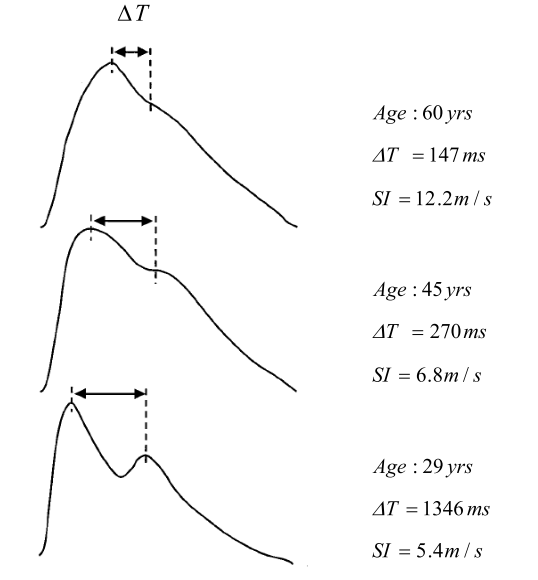
\includegraphics[width=.4\linewidth]{pulse_preprocess/si}
    \caption[SI计算原理示意]{\label{fig:si}SI计算原理示意\cite{Elgendi2012,Millasseau2002,Brumfield2005}}
\end{figure}

脉搏波波形速度(Pulse Wave Velocity,PWV)是指心脏每次搏动射血产生的沿大动脉壁传播的压力波传导速度\cite{Van2012}。在计算PWV时,需要在人体两部位分别测量脉搏波信号。
若记两测量部位的直线距离的80\%为$d$,两部位之间的脉搏波传导时间差为$t$,则有
\begin{equation}
    \label{equ:pwv}
    PWV = \frac{d}{t}
\end{equation}
PWV已被证实与动脉扩张性、僵硬度、管壁厚度和血液黏稠度密切相关。
特别地,PWV已经在子痫前期的诸多研究中得到应用\cite{Tomsin2012,Katsipi2014,VivianaIvan2018,Ira2014}。
需要注意的是,由于PWV的测量依赖于在人体不同部位测量脉搏波(且测量多利用压力传感器完成),故不适用单点测量的光电容积脉搏波研究。

\subsection{新型时域特征参数设计}
在总结前人研究基础上,本研究结合脉搏波形态特点,设计了多种新型时域描述参数,以求从新的角度完成对脉搏波波形特征的描述。

一、波形特征的设计基础

以纯数学的角度来看,PPG的信号波形可以近似描述为从一条往复于水平基线与波峰之间的双向路径。一般而言,PPG信号的上升支通常较下降支更为简单,该双向路径可以进一步简化为从波峰下降至水平基线的一条单向路径,只要完成对该单向路径的描述
即可类比完成上升支的描述,从而完成对整个脉搏波波形的描述,如\autoref{fig:road}所示。
\begin{figure}[htbp]
    \centering
    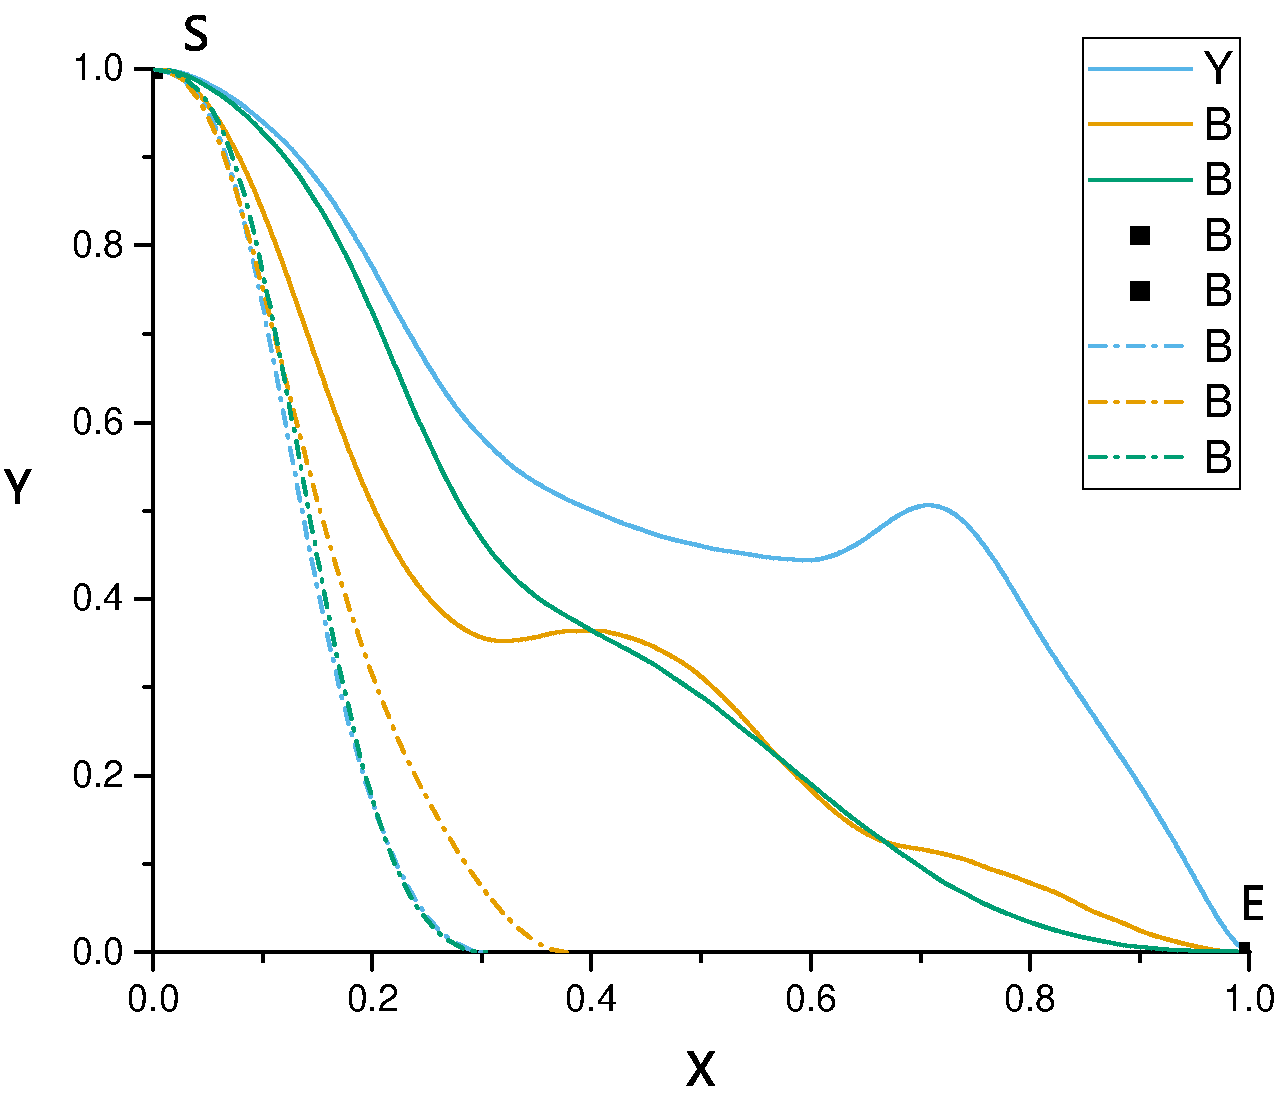
\includegraphics[width=.6\linewidth]{pulse_preprocess/road2}
    \caption[脉搏波波形的单向路径表示]{\label{fig:road}脉搏波波形的单向路径表示。其中三条路径由\autoref{fig:pulsecontrast}所示的同一被试的三段波形对应线形变换得来。同一颜色的实线部分与虚线部分对应同一个脉搏波的下降支与上升支
    ,其中,下降支按一定比例缩放至目标区间内,上升支水平反向按同一比例反向进行了缩放。}
\end{figure}

对上述路径的描述可通过对路径上点的描述来完成。不失一般性,我们可以将下降支的单向路径的起点坐标与终点坐标分别设置为S$(0,1)$与E$(1,0)$。对于该路径上任意一点P,可以用原点O坐标$(0,0)$与路径始末点坐标S、E等为基本参照点,以及P
在X轴、Y轴的投射点$P_x$、$P_y$等衍生参照点进行对该点进行描述,如\autoref{fig:point}所示。此时对P点进行描述可参考使用\autoref{tab:pointsdesc}中的参数指标,参数指标的归一化表达式也同时给出。
% 同一类型下关于起始S、E两点对偶的参数只保留了一个。
\begin{figure}[htbp]
    \centering
    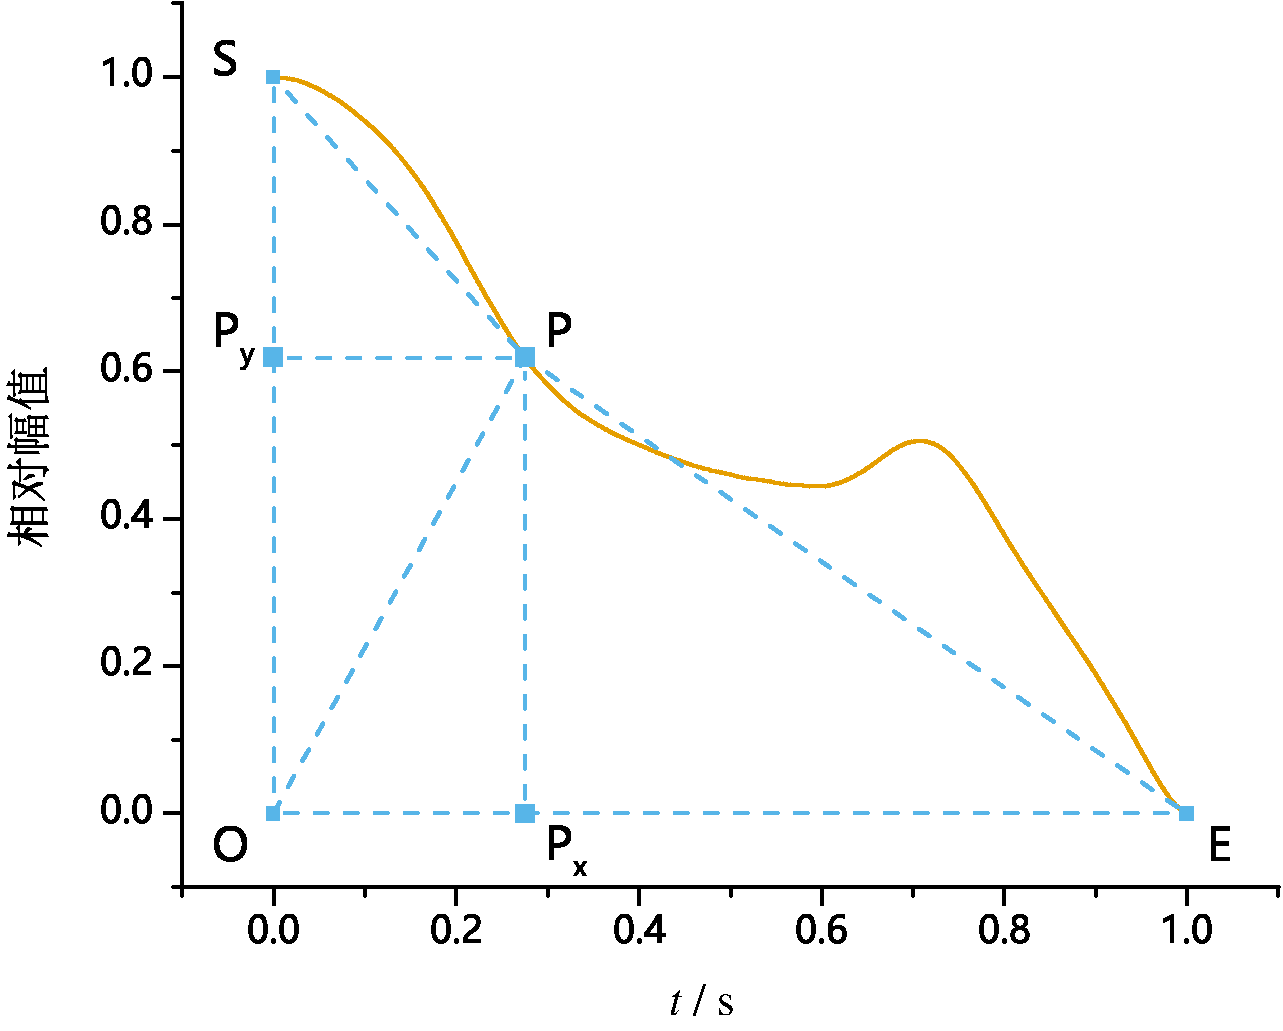
\includegraphics[width=.6\linewidth]{pulse_preprocess/point}
    \caption{\label{fig:point}单向路径上点的描述}
\end{figure}
\begin{center}
    \fontsize{10}{4}
    % Plan A
    % \setlength\LTleft{0pt}
    % \setlength\LTright{0pt}
	% \begin{longtable}{@{\extracolsep{\fill}}|c|c|c|c|c|}
    % Plan B
    % m表示居中,p为置顶,b为置底
    % 列宽总计16cm,各列按需分配长度,p{x-0.43cm}<{\centering}即可
    % \begin{longtable}{p{1.6cm}<{\centering}p{4.1cm}<{\centering}p{2.1cm}<{\centering}p{4.1cm}<{\centering}p{2.1cm}<{\centering}}
    \begin{longtable}{m{1.57cm}<{\centering}m{4.07cm}<{\centering}m{2.07cm}<{\centering}m{4.07cm}<{\centering}m{2.07cm}<{\centering}}
		\caption{单向路径上任意一点的描述指标一览}\\
		\label{tab:pointsdesc}\\
		\hline\hline
        \multirow{2}[2]{*}{\textbf{参数类型}} & \multicolumn{2}{c}{\textbf{原始数值表达}} & \multicolumn{2}{c}{\textbf{标准化表达}} \\
            & \multicolumn{1}{c}{物理意义} & \multicolumn{1}{c}{表达式或公式} & \multicolumn{1}{c}{物理意义} & \multicolumn{1}{c}{表达式或公式} \\
        \hline
        \endfirsthead
        \caption[]{(续)}\\
        \hline
        \multirow{2}[2]{*}{\textbf{参数类型}} & \multicolumn{2}{c}{\textbf{原始数值表达}} & \multicolumn{2}{c}{\textbf{标准化表达}} \\
            & \multicolumn{1}{c}{物理意义} & \multicolumn{1}{c}{表达式或公式} & \multicolumn{1}{c}{物理意义} & \multicolumn{1}{c}{表达式或公式} \\
        \hline
        \endhead 
        \hline
        \endfoot
        \hline\hline
        \endlastfoot
                                    & Y轴方向下降高度           &   $SP_y$      &  Y轴方向下降比例     & $\frac{SP_y}{OS}$ \\
                                    & P点高度                  &   $OP_y$       &    P点高度与波峰比值   & $\frac{OP_y}{OS}$ \\
                                    & 从S点到P点所用时间        &    $OP_x$   &      起点至P点所用时间与下降支总时长比值 & $\frac{OP_x}{OE}$ \\
                                    & 从P点到E点所用时间        &    $EP_x$   &      P点至终点E所用时间与下降支总时长比值 & $\frac{EP_x}{OE}$ \\
                                    & OP两点间几何距离        &    $OP$   &  OP两点距离与SE两点距离之比     & $\frac{OP}{SE}$ \\
                                    & SP两点间几何距离        &    $SP$   &  SP两点距离与SE两点距离之比     & $\frac{SP}{SE}$ \\
        \multirow{-7}*{线段}         & PE两点间几何距离        &    $PE$   &  PE两点距离与SE两点距离之比     & $\frac{PE}{SE}$ \\
                                    &  SP两点间曲线弧长     &  $L_{\overset{\frown}{SP}}$     &     SP两点间曲线弧长与SE两点直线距离之比  & $\frac{L_{\overset{\frown}{SP}}}{SE}$ \\
        \multirow{-2}*{曲线长度} &  PE两点间曲线弧长   &   $L_{\overset{\frown}{PE}}$    &    PE两点间曲线弧长与SE两点直线距离之比  &  $\frac{L_{\overset{\frown}{PE}}}{SE}$\\
                                    &  线段SP的斜率     &  $-\frac{SP_y}{PP_y}$     &   /    &  /  \\
                                    &  线段PE的斜率     &   $-\frac{P_yP_x}{EP_x}$    &    /  &  /   \\
        \multirow{-3}*{斜率(弧度)} &  线段OP的斜率    &    $\frac{PP_y}{PP_x}$   &    /   &  /     \\
                                    &  $\angle SPP_y$的弧度      & $\arctan(\frac{SP_y}{PP_y})$     &    /  &  /   \\
                                    &   $\angle POE$的弧度    &  $\arctan(\frac{P_yP_x}{EP_x})$      &    /  &  /   \\
        \multirow{-3}*{弧度(角度)}&   $\angle PEO$的弧度   &  $\arctan(\frac{PP_y}{PP_x})$         &    /  &  /   \\
                                    &    坐标轴、曲线与$PP_y$以上围成的面积   &  $\int_{P_y}^{S}{P(t)dy} $     &   前述面积与整体面积之比    & $\frac{\int_{P_y}^{S}{P(t)dy}}{\int_O^E{P(t)dx}}$ \\
                                    &   坐标轴、曲线与$OP$以左围成的面积   &    $\int_{O}^{P_x}{P(t)dx}-S_{\triangle OPP_x}$   &  前述面积与整体面积之比     & $\frac{\int_{O}^{P_x}{P(t)dx}-S_{\triangle OPP_x}}{\int_O^E{P(t)dx}}$ \\
                                    &   坐标轴、曲线与$PP_x$以左围成的面积   &   $\int_{O}^{P_x}{P(t)dx}$    &  前述面积与整体面积之比     & $\frac{\int_{O}^{P_x}{P(t)dx}}{\int_O^E{P(t)dx}}$ \\
        \multirow{-4}*{面积}        &    曲线与$SP$围成的面积   &   $\int_{P_y}^{S}{P(t)dy}-S_{\triangle SPP_y} $    &   /    &  /\\
	\end{longtable}
\end{center}

从\autoref{tab:pointsdesc}中不难发现,对于描述路径上的某一点来说,其线段指标、曲线长度指标、斜率指标及面积指标等是绑定在一起的。若以四者中某一指标的数值为具体标准,即可在路径上唯一确定与其绑定的数据点,此时按照定义即可对剩余指标进行描述。
考虑到实际计算难度,用线段指标或斜率指标来确定这样的数据点的过程是最容易实现的。此前诸多学者的提出的PPG描述指标也不外乎是这样的过程\cite{cwl,Wang2012,mmt}。

二、新型脉搏波时域特征

1. 脉搏波波形特征描述向量

特征描述向量是本研究为更准确描述刻画PPG波形周期内形态特点而提出一种描述方法。上小节出现的多项脉搏波时域参数往往是用一个数值来表征PPG波形形态,本研究中则使用了一组相互联系的数值来完成描述,这一过程可表示为
\begin{equation}
    \label{equ:featurevector}
    Feature_i=[v_0,v_1,\cdots,v_{n-1}]
\end{equation}

其中,特征描述向量的维数$n$可以在设计时人为指定。因此,之前的PPG时域参数可视为$n=1$的描述向量;若设定原始信号采样点数为$N$,则PPG原始数据可以视为$n=N$的描述向量;
预处理中对PPG信号进行插值处理后的数据可以视为$n>N$的超维描述向量。则显然随着维数的增加,向量对原始脉搏波的描述能力越强。这一现象可以用信息论中的编码理论进行解释,即通讯过程中在信源原始符号不变的情况下,
增加变换编码的输出符号长度可以提高系统的信息传输能力\cite{Zhao2017}。故特征描述向量是变换编码下的一种编码长度与信息描述能力的折中。

此外,由于本研究特征向量的维数一般在x附近。针对全部向量内元素为

2、双向均一化与膨胀-腐蚀指数

双向均一化法是本研究使用的一种量化比较峰值、周期均不相同的脉搏波波形形态特征的处理方法。如前文波形特征的设计基础小节介绍,若将两条路径所对应的原始脉搏波的波峰、下降支时长均映射至$[0,1]$区间内,此时即可评估
该两条路径的相似度,如\autoref{fig:road}所示。若两条路径完全重合,则说明两个脉搏波下降支波形有着峰值、周期以外的共性特征。针对更一般的不重合的两条路径,本研究利用幂函数簇的相关性质,首创提出了膨胀-腐蚀指数
(erode and dilate index,EDI)这一新特征参数以表征描述其形态特征。
\begin{figure}[h]
    \centering
    \subfigure[\label{fig:pow}幂函数簇在0<x<1区间内图像。]{
    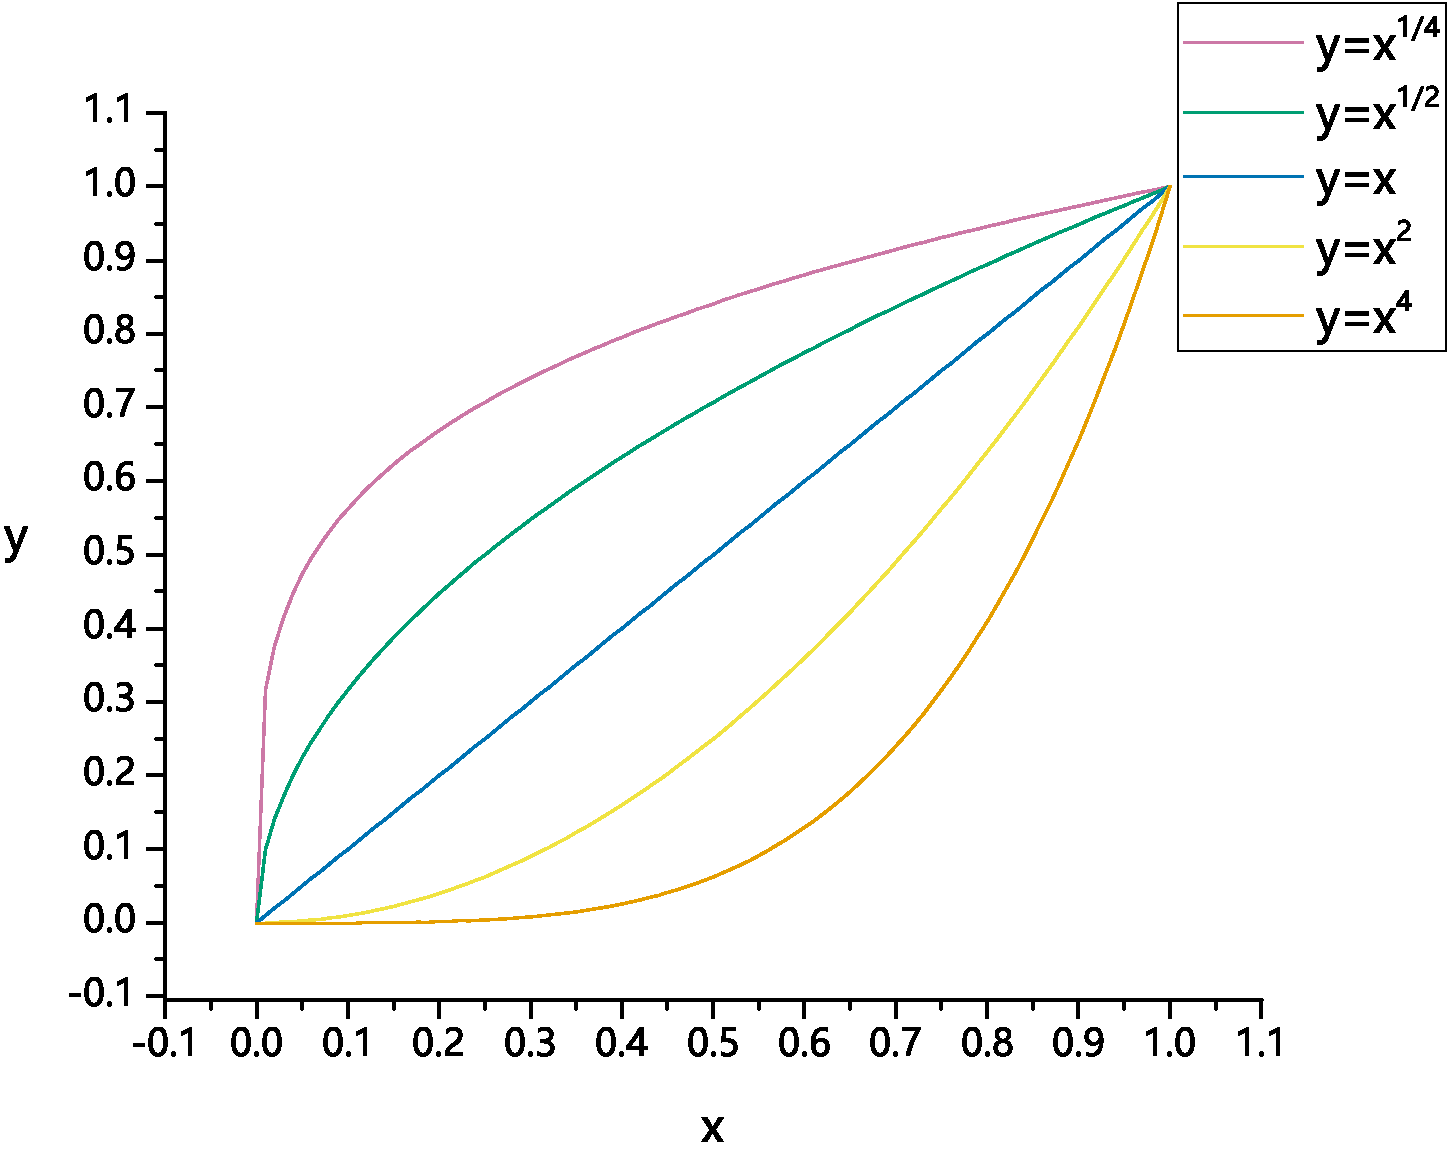
\includegraphics[width=5.5cm]{pulse_preprocess/pow}
    }
    \quad
    \subfigure[\label{fig:edi1}对\autoref{fig:pulsecontrast}中脉搏波波形进行EDI计算 I]{
    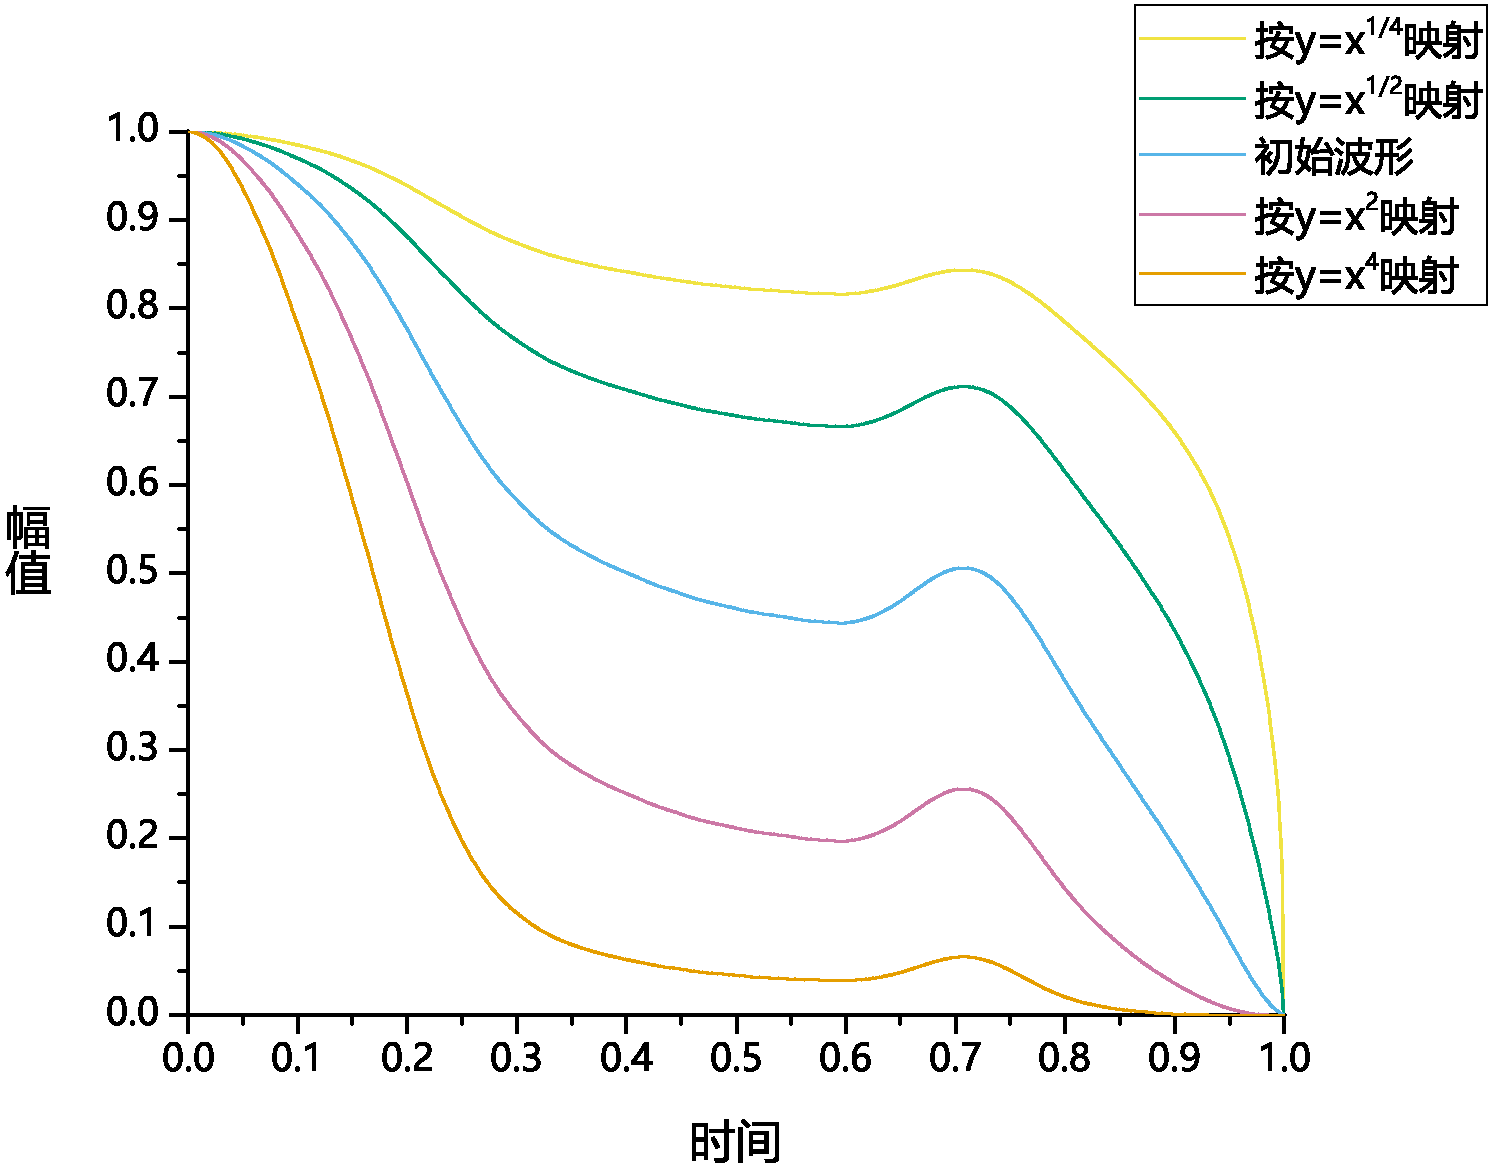
\includegraphics[width=5.5cm]{pulse_preprocess/edi1}
    }
    \quad
    \subfigure[\label{fig:edi2}对\autoref{fig:pulsecontrast}中脉搏波波形进行EDI计算 II]{
    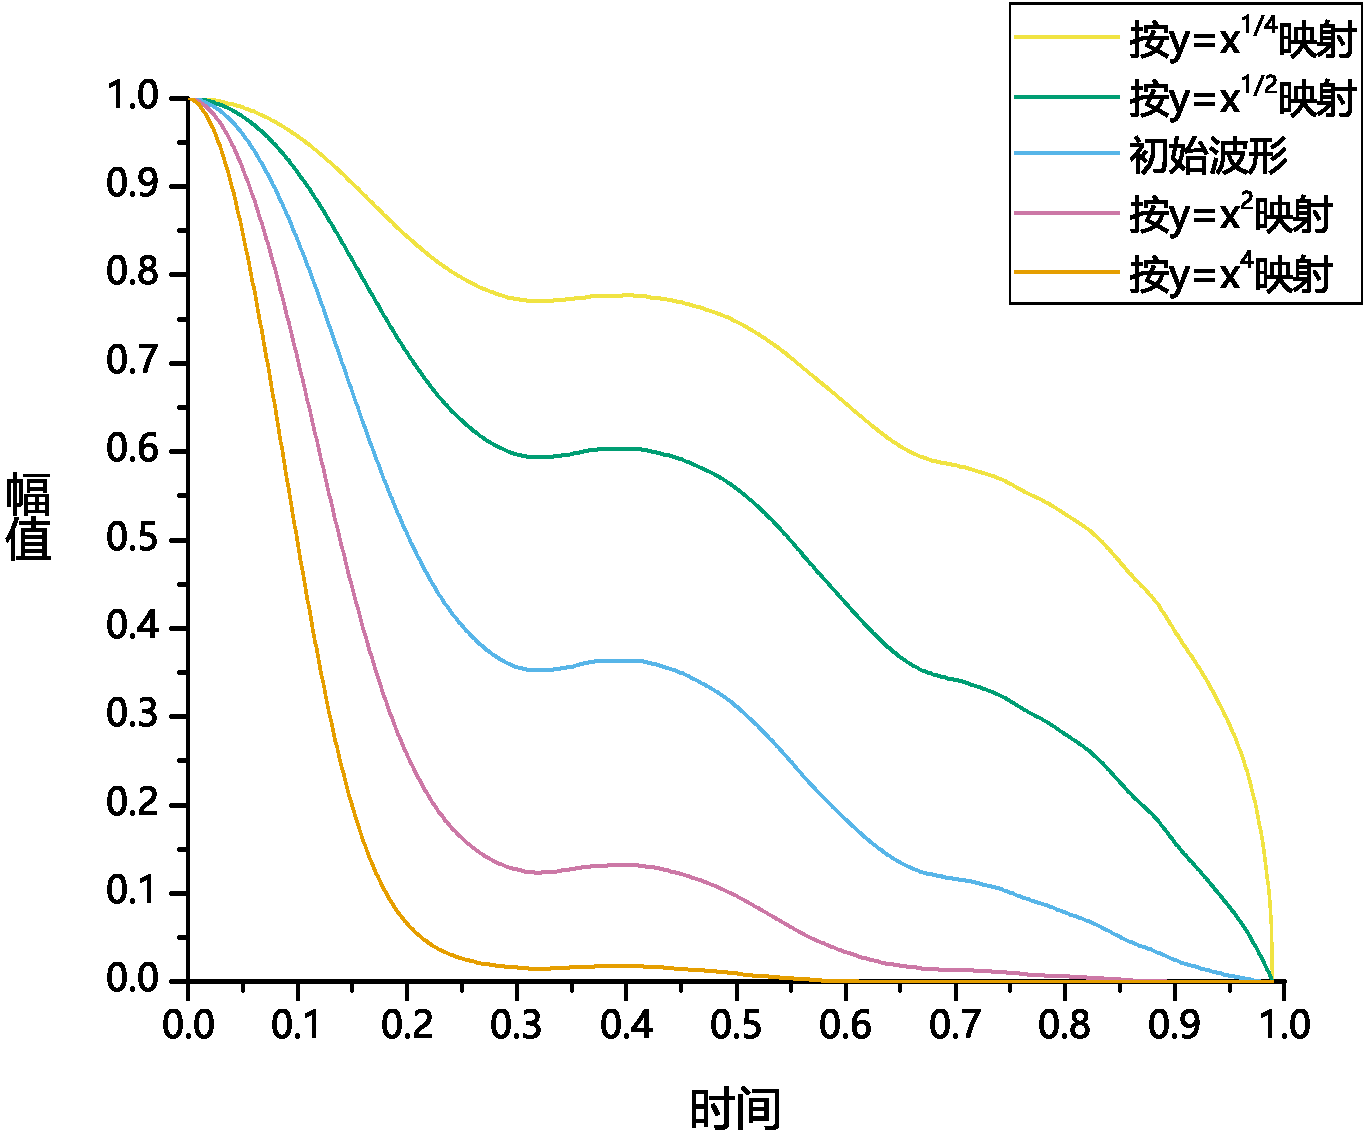
\includegraphics[width=5.5cm]{pulse_preprocess/edi2}
    }
    \quad
    \subfigure[\label{fig:edi3}对\autoref{fig:pulsecontrast}中脉搏波波形进行EDI计算 III]{
    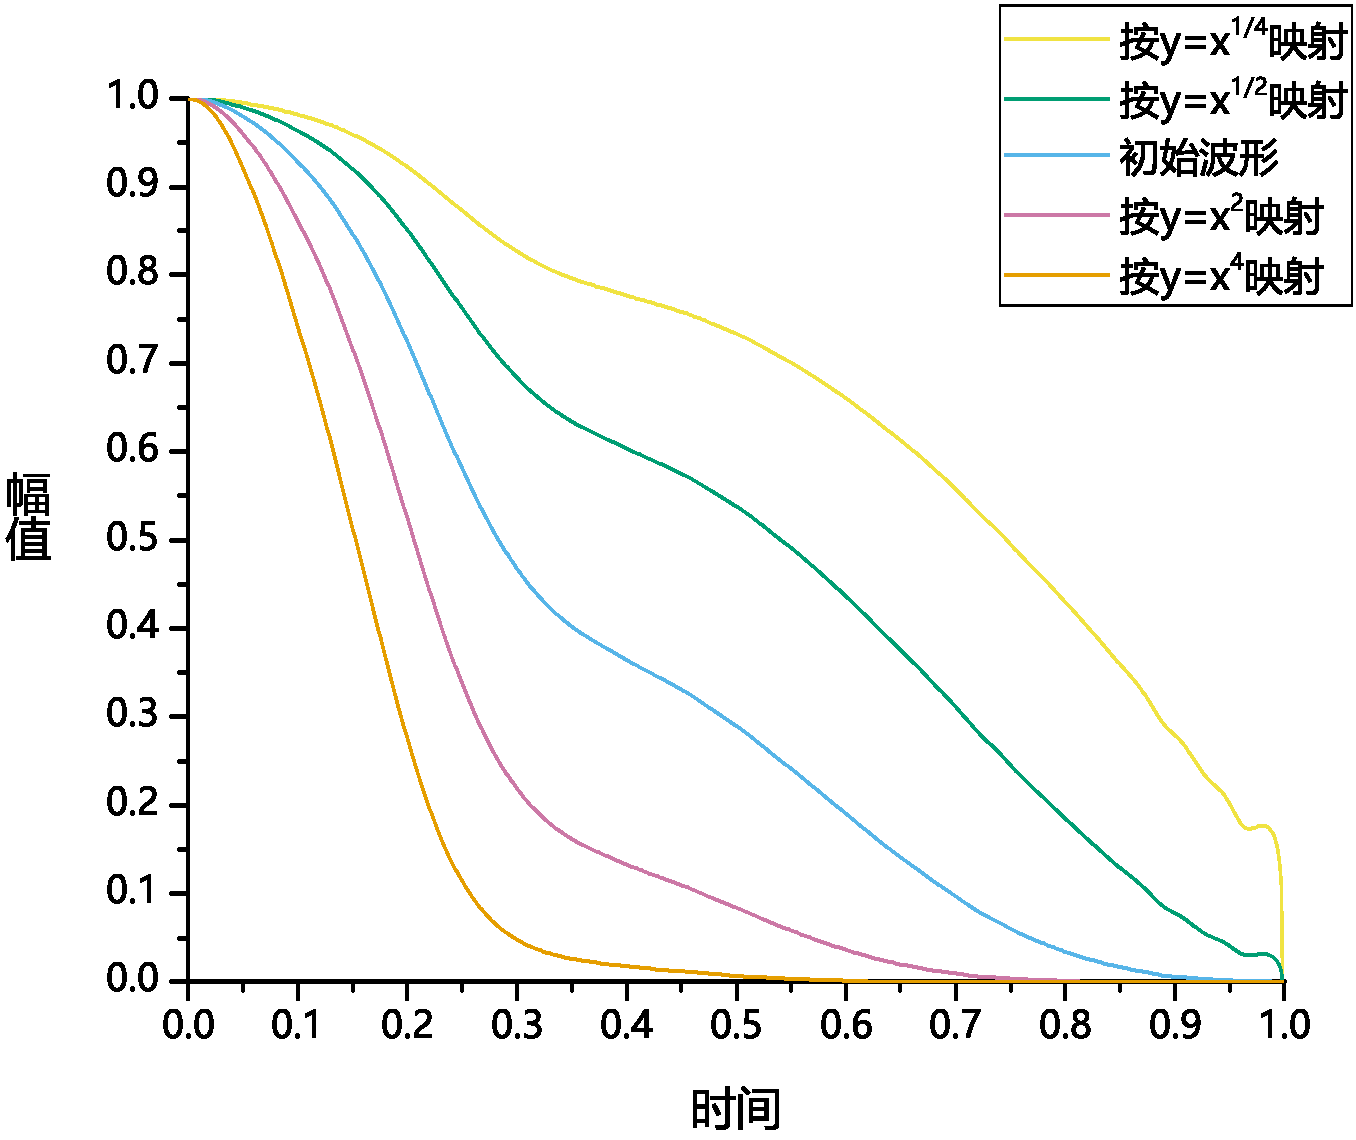
\includegraphics[width=5.5cm]{pulse_preprocess/edi3}
    }
    \caption{\label{fig:powandedi}幂函数簇与PPG波形的EDI指标示意}
\end{figure}

% \begin{figure}[htbp]
%     \centering
%     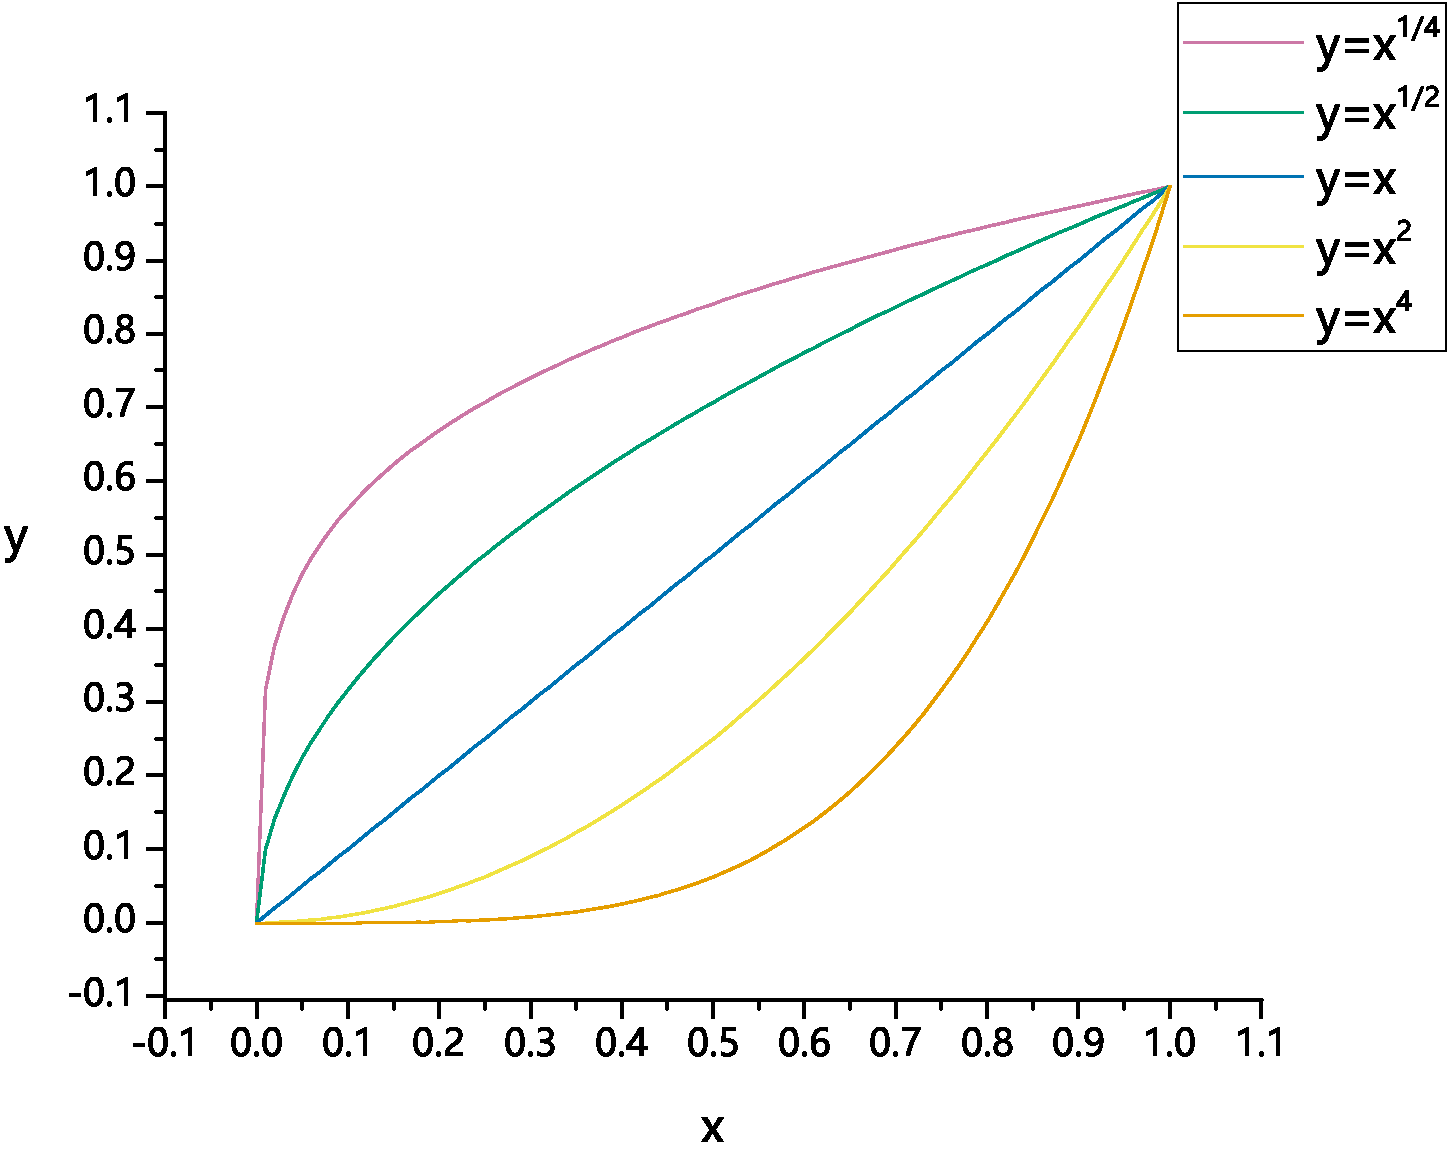
\includegraphics[width=.6\linewidth]{pulse_preprocess/pow}
%     \caption[幂函数簇的图像(局部)]{\label{fig:pow}幂函数簇在$[0,1]$区间内图像。图形自上而下依次为$y=x^{\frac{1}{4}}$、$y=x^{\frac{1}{2}}$、$y=x$、$y=x^2$及$y=x^4$。}
% \end{figure}

考察$f(x)=x^n$幂指数函数簇的相关数学性质,可知幂函数簇在定义域内均保持单调递增的性质,若限定函数定义域$x\subseteq [0,1]$,对于$n>1$的幂指数函数,$f(x)$均在$y=x$图像的下方,且$n$值越大,图像越贴近$x$轴,
函数图像“腐蚀”得越发严重;反之,$0<n<1$的幂指数函数会使$y=x$的图像趋近于直线$x=1$,$n$值越大,函数图像“膨胀”得愈益明显,如\autoref{fig:pow}所示。
换言之,若给定某一具体的定义域与值域均在$[0,1]$的函数$g(x)$,
在其原始函数映射关系的基础上进一步使用任一幂函数($n\neq 1$)进行二次映射,即可在不改变值域的条件下对原始$g(x)$图像进行非线性缩放。幂函数对原始函数中不同数值均有着不同的缩放比例,即可以在一定程度上反应原始数值的分布
特性。此外,由于幂函数本身的单调性可以保证这样的非线性缩放结果也是唯一的。此时对原始函数$g(x)$的描述即可转换成对该非线形缩放过程的描述,并可进一步转换成对函数图像膨胀、腐蚀程度的描述,如\autoref{fig:edi1}-\autoref{fig:edi3}所示。

参照上小节的面积类参数原理,若将双向均一化后的下降支与坐标轴围成的面积记为$S_{bn}$,同理经幂函数$f(x)=x^i$二次映射后的图形面积记为$S_{bn-i}$,则两者的差值可记为
\begin{equation}
    \label{equ:sbn}
    \Delta S_{bn-i}=S_{bn}-S_{bn-i}
\end{equation}
本研究在实际计算时选取了$f(x)=x^2$与$f(x)=x^{\frac{1}{2}}$两个基底幂函数进行计算,并将最后的EDI也以向量形式记为
\begin{equation}
    \label{equ:edi}
    EDI=[S_{bn},S_{bn-2},\Delta S_{bn-2},S_{bn-\frac{1}{2}},\Delta S_{bn-\frac{1}{2}}]
\end{equation}

需要注意的是,在脉搏波双向均一化过程中,幅值方向的均一化处理易于理解也较容易完成,但在时长尺度的处理上,直接均一化很可能导致即使完全相同的波形也会因为原始数据的采样点数目不同而导致结果迥异。因此,时间均一化过程
需保证最后所有波形下降支的数据采样点数目一致。在实际处理时,本研究舍弃了PPG波形的原始采样值,使用三次样条插值方法将下降支原始波形的采样点数均匀插值提高至1000,最后将所有数值映射到$[0,1]$区间。

\subsection{PPG时域描述特征集构建}
本小节对本研究实际采用的多种PPG时域描述特征进行汇总,对各参数符号及前置计算条件也进行了统一说明,如\autoref{tab:allfeatures}所示。
TODO
\begin{center}
    \fontsize{10}{4}
	\begin{longtable}{p{3cm}<{\centering}p{1cm}<{\centering}p{2cm}<{\centering}p{6cm}<{\centering}p{1cm}<{\centering}}
		\caption{本研究使用的所有PPG时域指标一览}\\
		\label{tab:allfeatures}\\
		\hline\hline
            \textbf{研究者}&\textbf{时间}&\textbf{脉搏波参数}&\textbf{研究结果}&\textbf{备注}\\
        \hline
        \endfirsthead
        \caption[]{(续)}\\
        \hline
            \textbf{研究者}&\textbf{时间}&\textbf{脉搏波参数}&\textbf{研究结果}&\textbf{备注}\\
        \hline
        \endhead 
        \hline
        \endfoot
        \hline\hline
        \endlastfoot
        &       &       &       &  \\
        &       &       &       &  \\
        &       &       &       &  \\
        &       &       &       &  \\
        &       &       &       &  \\
	\end{longtable}
\end{center}
\subsection{脉搏波的直接描述}
\subsection{脉搏波间的描述与度量}
包络线

Frechet Distance

\begin{figure}[htbp]
    \centering
    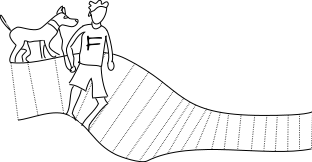
\includegraphics[width=.6\linewidth]{pulse_preprocess/frechet_distance}
    \caption{\label{fig:frechet distance}frechet distance}
\end{figure}

互相关系数
\section{小结}
本章主要对脉搏波信号的预处理过程与参数描述进行了详细了的说明。预处理方面,本研究重点介绍了经改进的模块化脉搏波的定位算法,该算法可以有效识别干扰段,提高检测精度。随后对信号滤波、重搏波检测、基线漂移、插值及标准化过程进行了介绍。
脉搏波的描述方面,首先介绍了脉搏波描述的意义,其次从基于波形与基于时间窗等两大类,分别介绍了常见的脉搏波时域参数与本研究提出的新型描述参数,并在两者的基础上构建了脉搏波的一般时域特征描述集合,为后续数据分析部分打下坚实的基础。